\documentclass[9pt,handout,aspectratio=169]{beamer}

\usepackage{pgfnodes}
\usepackage{pgfpages}
\usepackage{color}
\usepackage{hyperref}
\usepackage{xspace}
\usepackage[absolute,overlay]{textpos}

\input{/home/rustem/talks/figures/commands.tex}

\setbeamertemplate{footline}[frame number]

\mode<presentation>{\usetheme{default}}

\setbeamertemplate{footline}[text line]
{\parbox{\linewidth}{\vspace*{-8pt}Summary of some of the recent climate observations \& predictions \hfill\insertshortauthor\hfill\insertpagenumber}}
\setbeamertemplate{navigation symbols}{}

\title{}
\author{Rustem Ospanov}

%%%%%%%%%%%%%%%%%%%%%%%%%%%%%%%%%%%%%%%%%%%%%%%%%%%%%%%%%%%%%%%%%%%%%%%%%%%%%%%%%%
\begin{document}

%%%%%%%%%%%%%%%%%%%%%%%%%%%%%%%%%%%%%%%%%%%%%%%%%%%%%%%%%%%%%%%%%%%%%%%%%%%%%%%%%%
%%%%%%%%%%%%%%%%%%%%%%%%%%%%%%%%%%%%%%%%%%%%%%%%%%%%%%%%%%%%%%%%%%%%%%%%%%%%%%%%%%

%%%%%%%%%%%%%%%%%%%%%%%%%%%%%%%%%%%%%%%%%%%%%%%%%%%%%%%%%%%%%%%%%%%%%%%%%%
%%%%%%%%%%%%%%%%%%%%%%%%%%%%%%%%%%%%%%%%%%%%%%%%%%%%%%%%%%%%%%%%%%%%%%%%%%
\begin{frame}
  \begin{small}
              
  \begin{columns}
  \column{0.9\textwidth}
  \hhref{https://public.wmo.int/en/our-mandate/climate/wmo-statement-state-of-global-climate}{State of Global Climate 2021} report prepared by World Meteorological Organisation (WMO)
    \begin{itemize}\setlength\itemsep{2.0ex}\footnotesize
      \item[o] Annual report detailing the global climate in 2021, including historical comparisons and trends
    \end{itemize}
  \end{columns}

  \end{small}
  \end{frame}

%%%%%%%%%%%%%%%%%%%%%%%%%%%%%%%%%%%%%%%%%%%%%%%%%%%%%%%%%%%%%%%%%%%%%%%%%%%%%%%%%%
\begin{frame}
  \frametitle{\centerline{ \hhref{https://public.wmo.int/en/our-mandate/climate/wmo-statement-state-of-global-climate}{State of Global Climate 2021:} global temperature and CO$_2$ emissions}}
  \begin{scriptsize}

    \begin{columns}
      \column{1.0\textwidth}
      \begin{itemize}\setlength\itemsep{1.3ex}
        \item[o] {\cb Left:} Average global CO$_2$ concentration (parts per million) from 1984 to 2020. The red line is the monthly mean without seasonal variations.

        \item[o] {\it Increasing levels of CO$_2$ and other greenhouse gases in the atmosphere are a major driver of climate change.} Atmospheric CO$_2$ concentrations reflect a balance between emission sources and sinks. Raising global CO$_2$ concentrations reflect the budget between extra emissions due to human activities and uptake by the biosphere and ocean.

        \item[o] {\cb Right:} Mean global temperature from 1850 to 2021. The global temperature in 2021 was $1.11 \pm 0.13~^{\circ}$C above the 1850-1900 average. The six data sets place 2021 between the 5th and 7th warmest year on record. {\it The seven warmest years on record were between 2015 and 2021.}
      \end{itemize}
    \end{columns}

    \begin{columns}

      \column{0.40\textwidth}
        \begin{center}
        {\scriptsize \cb Average global CO$_2$ concentration}
          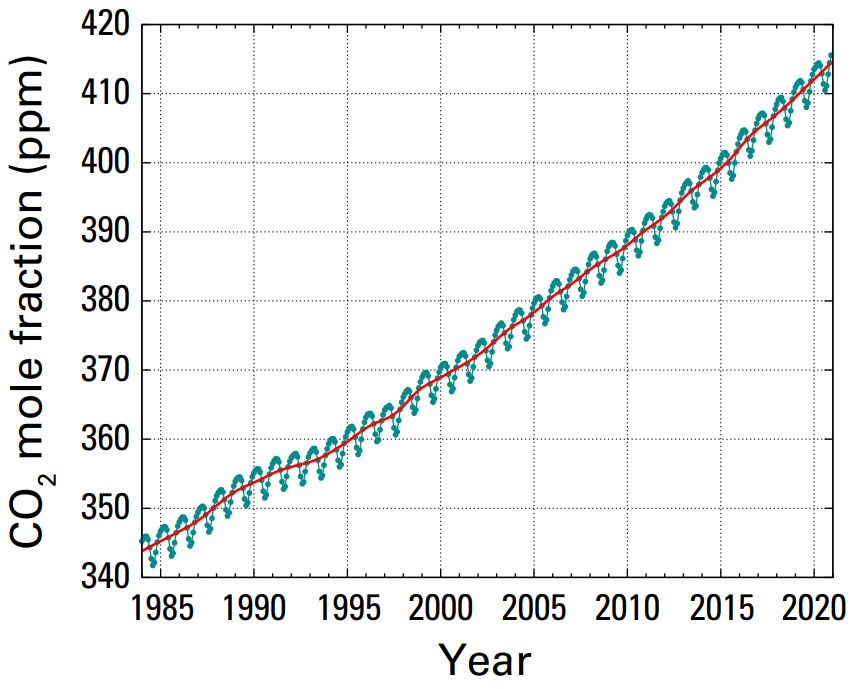
\includegraphics[width=1.0\textwidth]{plots/WMO_CO2}
        \end{center}

      \column{0.65\textwidth}
      \begin{center}
        {\scriptsize \cb Average global temperature change with respect to the 1850-1900 average}
          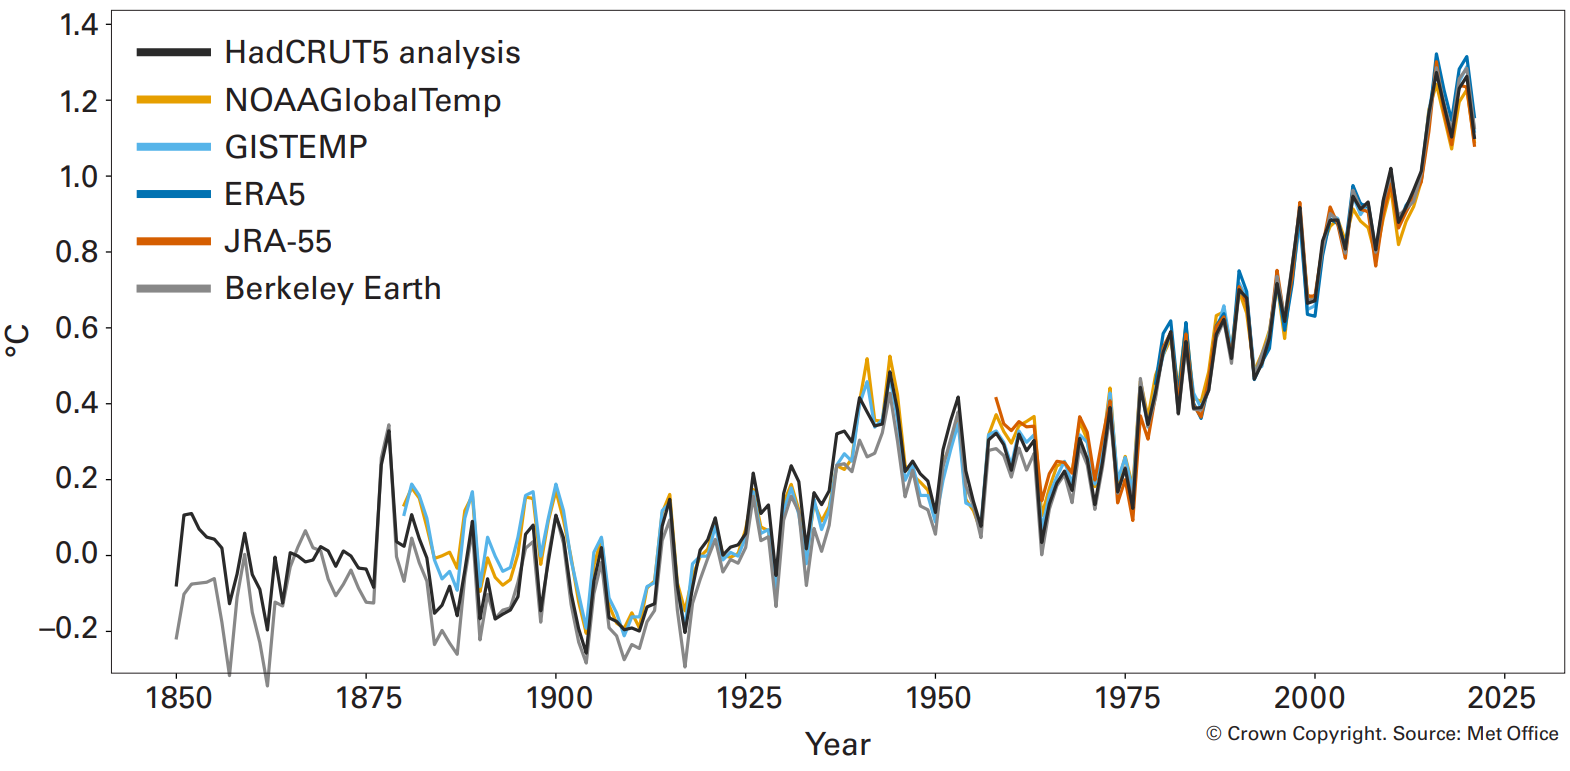
\includegraphics[width=1.0\textwidth]{plots/WMO_temperature}
      \end{center}
    \end{columns}

  \end{scriptsize}
  \end{frame}


%%%%%%%%%%%%%%%%%%%%%%%%%%%%%%%%%%%%%%%%%%%%%%%%%%%%%%%%%%%%%%%%%%%%%%%%%%%%%%%%%%
\begin{frame}
  \frametitle{\centerline{ \hhref{https://public.wmo.int/en/our-mandate/climate/wmo-statement-state-of-global-climate}{State of Global Climate 2021:} average near-surface temperature in 2021}}
  \begin{scriptsize}

    \begin{columns}
      \column{1.0\textwidth}
      \begin{itemize}\setlength\itemsep{1.3ex}
        \item[o] Map of the near-surface temperatures in 2021 compared to the 1981-2010 average. Near-surface temperatures in 2021 were above 1981-2010 average across a broad swath of North America and Greenland, Northern and Tropical Africa, the Middle East and Southern Asia.
        
        \item[o] Cooler conditions in Southern Africa, India, and eastern Australia are characteristic of La Niña. The cooler-than-average area in Northern Asia stands in contrast to 2020, which saw exceptionally high temperatures in the region.

        \item[o] \hhref{https://climate.copernicus.eu/temperature-animations}{Link to animation of year-to-year variations in surface air temperature}
      \end{itemize}
    \end{columns}

    \begin{columns}
      \column{0.7\textwidth}
      \begin{center}
          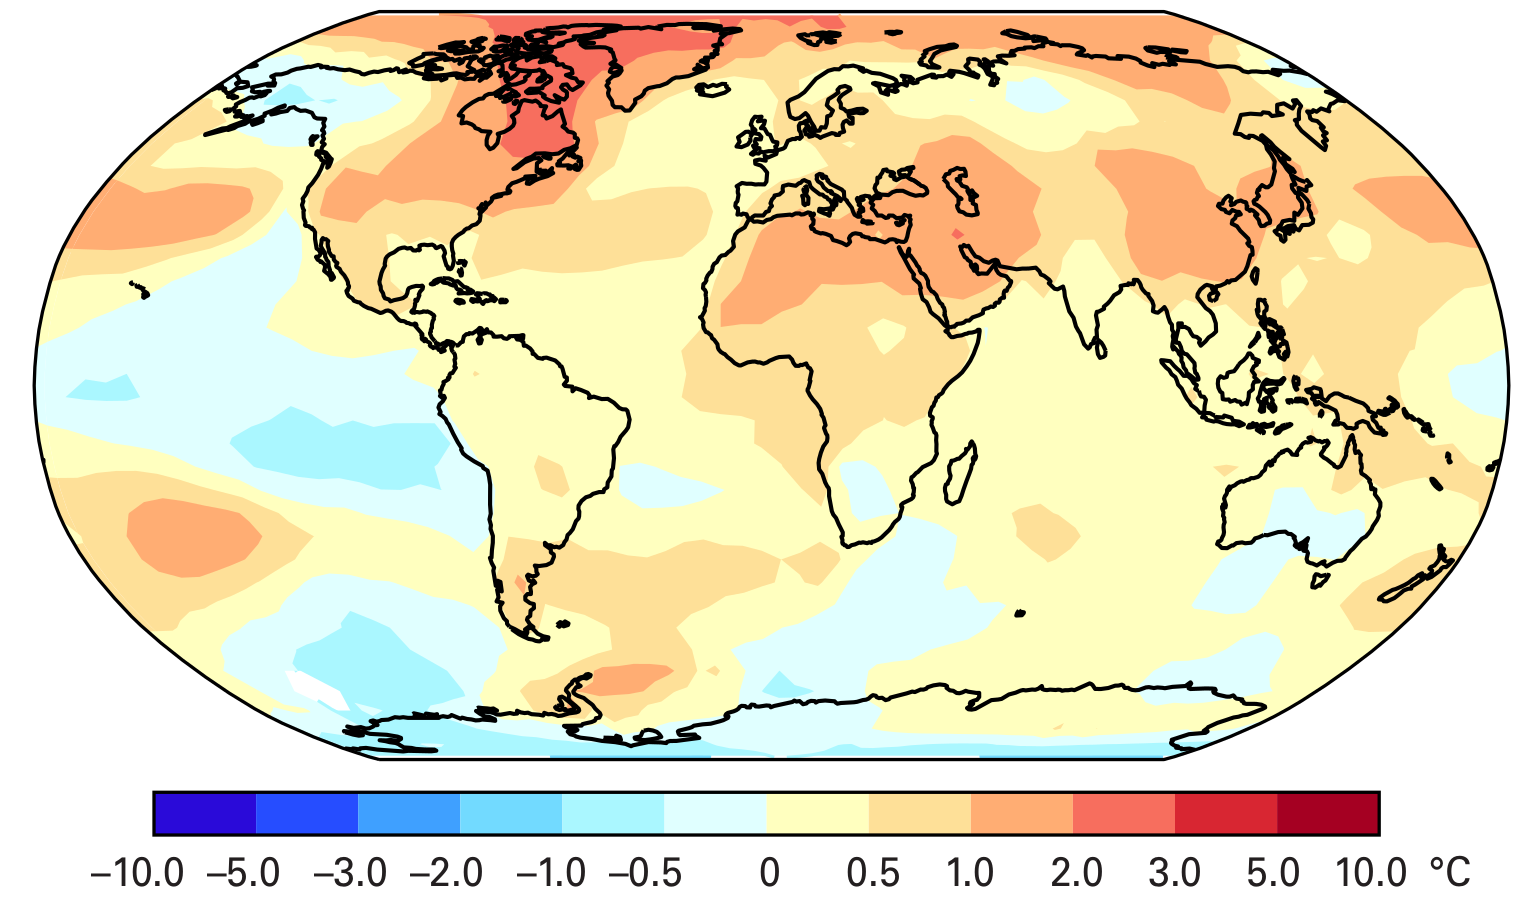
\includegraphics[width=1.0\textwidth]{plots/WMO_temperature_map}
      \end{center}
    \end{columns}

  \end{scriptsize}
  \end{frame}

%%%%%%%%%%%%%%%%%%%%%%%%%%%%%%%%%%%%%%%%%%%%%%%%%%%%%%%%%%%%%%%%%%%%%%%%%%%%%%%%%%
\begin{frame}
  \frametitle{\centerline{ \hhref{https://public.wmo.int/en/our-mandate/climate/wmo-statement-state-of-global-climate}{State of Global Climate 2021:} melting of ice sheets}}
  \begin{scriptsize}

    \begin{columns}
      \column{1.0\textwidth}
      \begin{itemize}\setlength\itemsep{1.3ex}
        \item[o] The average annual rate of ice mass loss from 2002 to 2018 was 276 gigatonne in Greenland and 152 gigatonne in Antarctica, measured with GRACE and GRACE-FO satellite gravity data.        
        \item[o] {\it This is equivalent to about 1.2 mm per year of the global sea-level rise.}

        \item[o] Over the past 30 years, the number of people living in  high risk coastal areas due to rising sea levels increased from 160 million to 260 million.
      \end{itemize}

    \end{columns}

    \vspace{0.2cm}
    \begin{columns}
      \column{1.05\textwidth}
      \begin{center}
          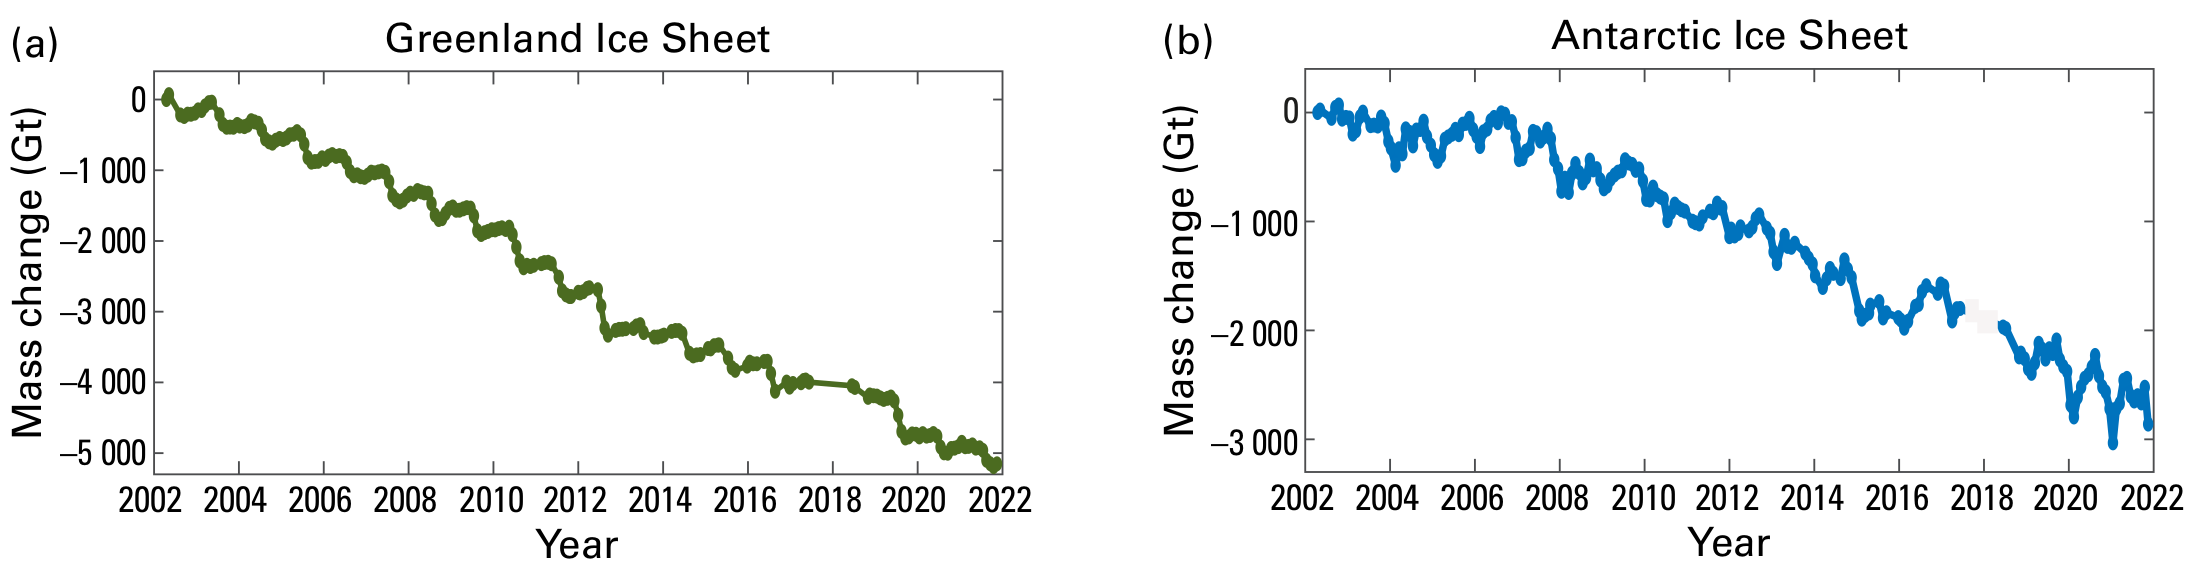
\includegraphics[width=1.0\textwidth]{plots/WMO_ice_sheets}
      \end{center}
    \end{columns}

  \end{scriptsize}
  \end{frame}


%%%%%%%%%%%%%%%%%%%%%%%%%%%%%%%%%%%%%%%%%%%%%%%%%%%%%%%%%%%%%%%%%%%%%%%%%%%%%%%%%%
\begin{frame}
  \frametitle{\centerline{ \hhref{https://public.wmo.int/en/our-mandate/climate/wmo-statement-state-of-global-climate}{State of Global Climate 2021:} see level raise and ocean heat content}}
  \begin{scriptsize}

    \begin{columns}
      \column{1.0\textwidth}
      \begin{itemize}\setlength\itemsep{1.3ex}
        \item[o] {\cb Left:} Global mean sea level evolution from January 1993 to January 2022 (black curve) based on high-precision satellite altimetry. The coloured straight lines represent the average linear trend over three successive time spans: 1993-2002; 2003-2012; 2013-2022.

        
        \item[o] {\cb Right:} Global mean ocean heat content relative to 1955 for depths of 0 to 700~meters in light blue and 700 to 2000~meters in dark blue. 

        \item[o] Oceans cover about 70\% of the earth's surface and have high capacity to absorb extra heat trapped by the CO$_2$ and other greenhouse gases. {\it The ocean takes up more than 90\% of the excess energy accumulating in the Earth climate system as a result of increased concentrations of greenhouse gases.} Melting of ice sheets and thermal expansion of warming oceans lead to a sea level rise, impacting coastlines. Rising CO$_2$ concentrations in the atmosphere change ocean chemistry, causing acidification of the oceans, with negative consequences for marine biosphere.

      \end{itemize}
    \end{columns}

    \begin{columns}
      \column{0.49\textwidth}
      \begin{center}
        {\scriptsize \cb Accelerating raise of the global sea level}
          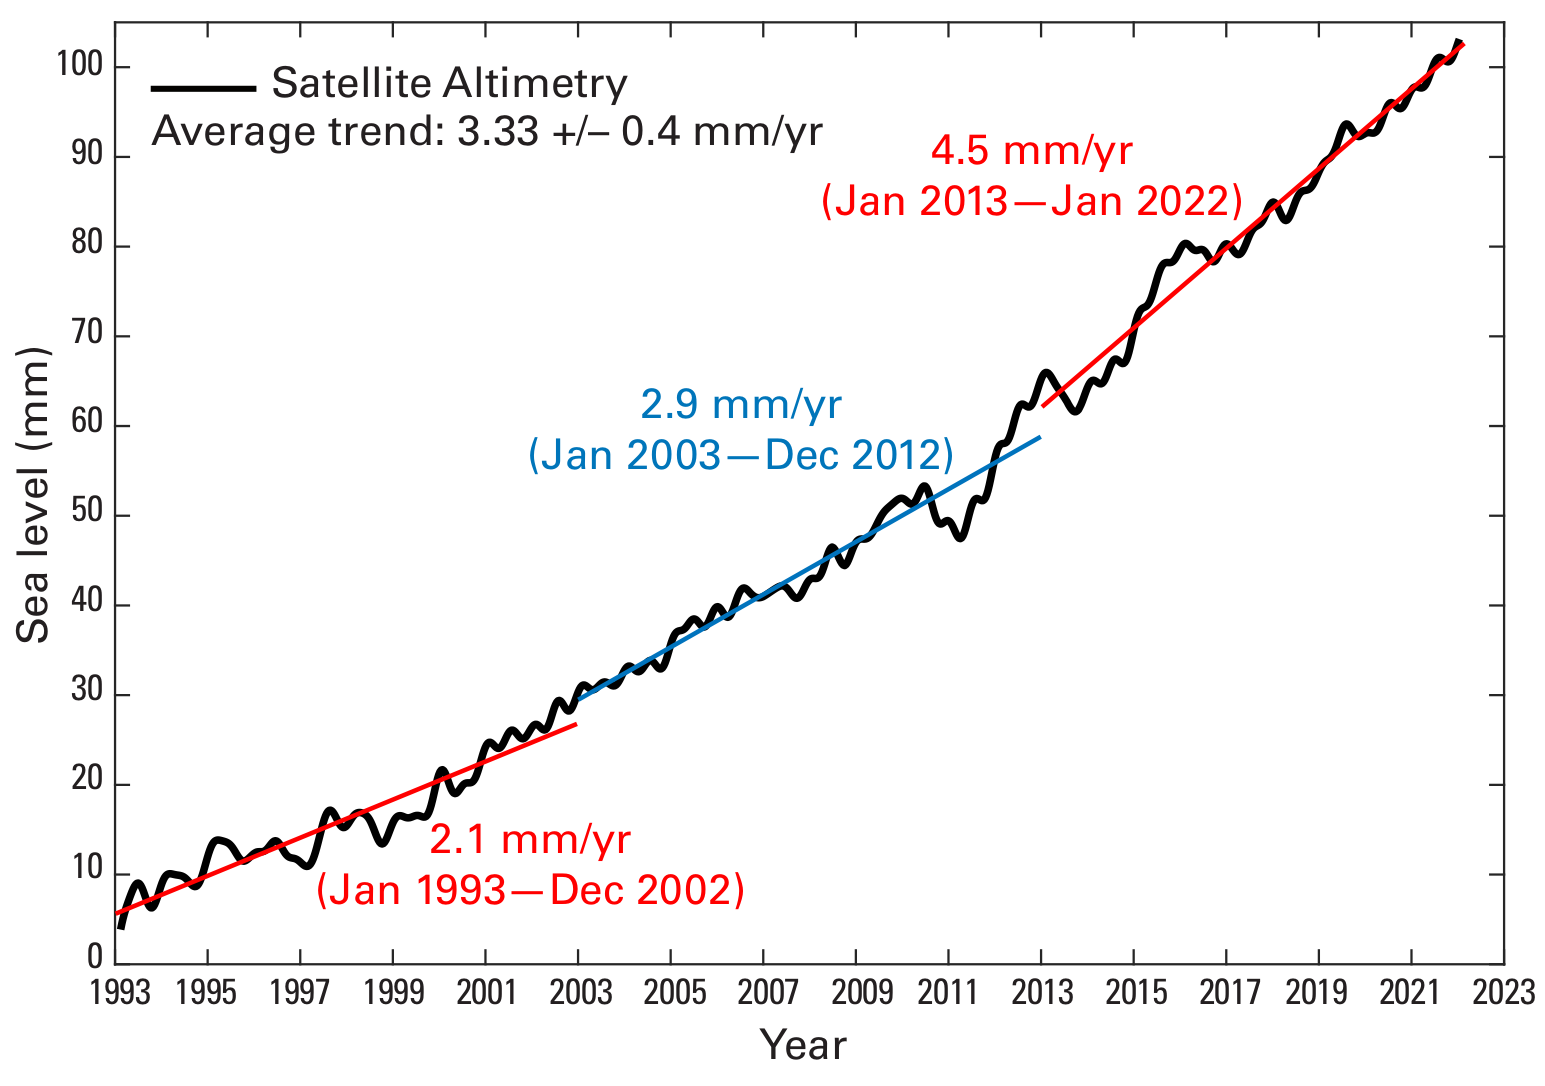
\includegraphics[width=1.0\textwidth]{plots/WMO_sea_level}
      \end{center}

      \column{0.49\textwidth}
      \begin{center}
        {\scriptsize \cb Increasing heat content of the oceans}
          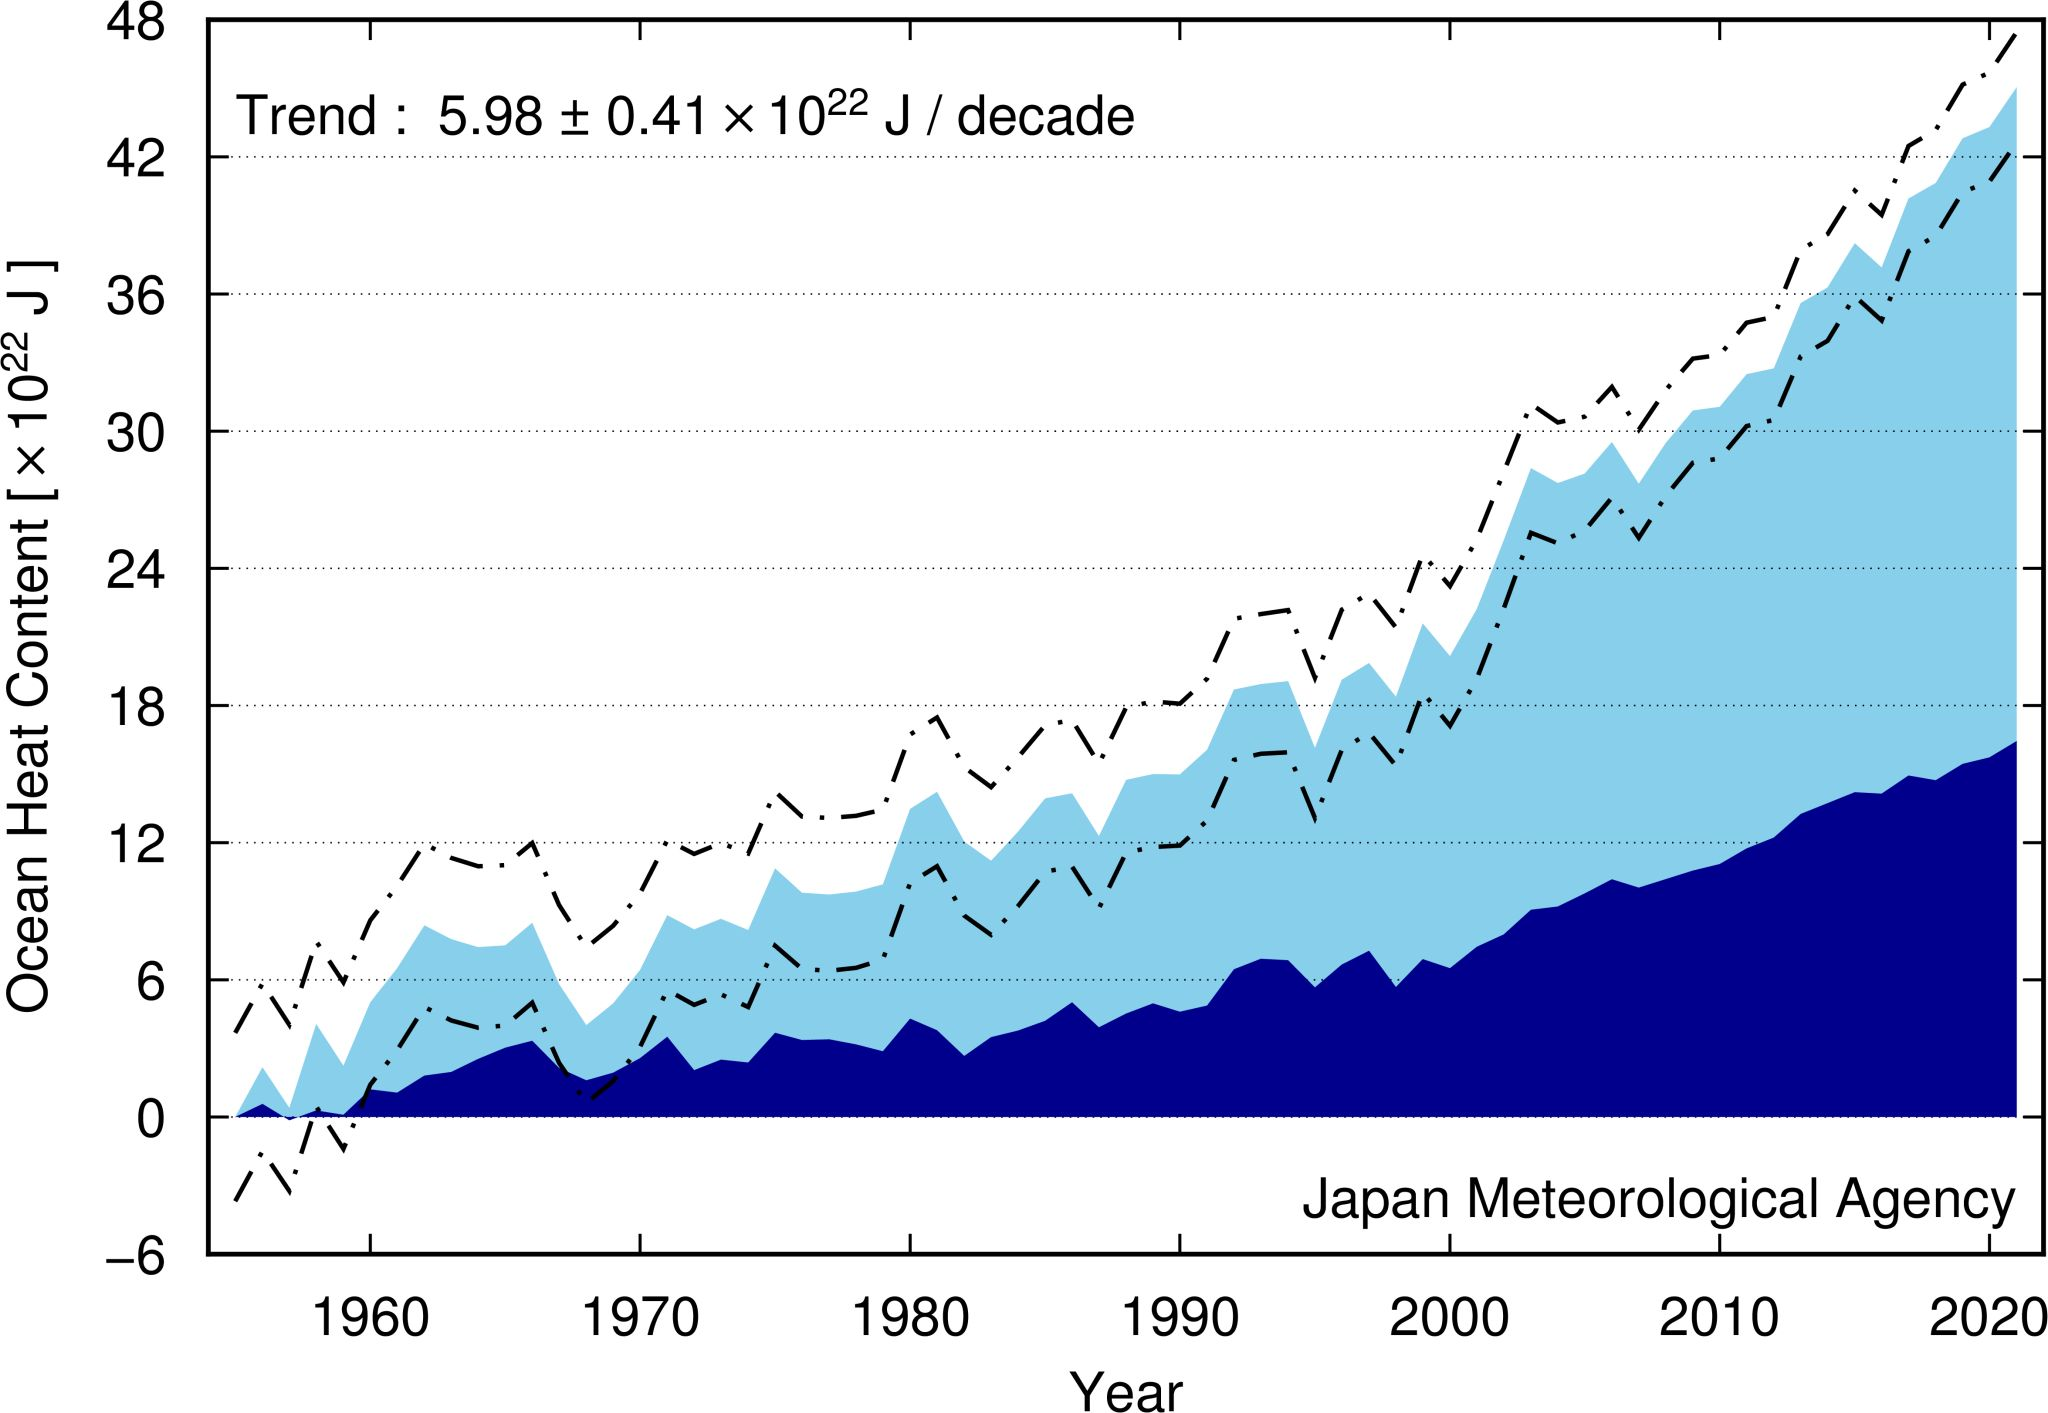
\includegraphics[width=1.0\textwidth]{plots/JMO_sea_heat}
      \end{center}      
    \end{columns}

  \end{scriptsize}
  \end{frame}


%%%%%%%%%%%%%%%%%%%%%%%%%%%%%%%%%%%%%%%%%%%%%%%%%%%%%%%%%%%%%%%%%%%%%%%%%%%%%%%%%%
%%%%%%%%%%%%%%%%%%%%%%%%%%%%%%%%%%%%%%%%%%%%%%%%%%%%%%%%%%%%%%%%%%%%%%%%%%%%%%%%%%


%%%%%%%%%%%%%%%%%%%%%%%%%%%%%%%%%%%%%%%%%%%%%%%%%%%%%%%%%%%%%%%%%%%%%%%%%%
%%%%%%%%%%%%%%%%%%%%%%%%%%%%%%%%%%%%%%%%%%%%%%%%%%%%%%%%%%%%%%%%%%%%%%%%%%
\begin{frame}
  \begin{small}
              
  \begin{columns}
  \column{0.9\textwidth}
  {\cb Intergovernmental Panel on Climate Change (IPCC) Assessment Report 6 (2021)}
    \begin{itemize}\setlength\itemsep{1.0ex}\footnotesize
      \item[1.]  \hhref{https://www.ipcc.ch/report/ar6/wg1/downloads/report/IPCC_AR6_WGI_SPM_final.pdf}{IPCC Working Group I: Physical Science Basis}
    \end{itemize}
  \end{columns}

  \end{small}
\end{frame}  

%%%%%%%%%%%%%%%%%%%%%%%%%%%%%%%%%%%%%%%%%%%%%%%%%%%%%%%%%%%%%%%%%%%%%%%%%%%%%%%%%%
\begin{frame}
  \frametitle{\centerline{\hhref{https://www.ipcc.ch/report/ar6/wg1/downloads/report/IPCC_AR6_WGI_SPM_final.pdf}{IPCC Physical Science Basis:} Temperature trends with/without impact of human activity}}
  \begin{scriptsize}

    \begin{columns}
      \column{1.0\textwidth}
      \begin{itemize}\setlength\itemsep{1.9ex}        
        \item[o] {\cb Left:} Human influence has warmed the climate at a rate that is unprecedented in at least the last 2000 years. Current global temperature trends are comparable to the warmest multi-century period in more than 100,000 years.

        \item[o] {\cb Right:} Observed changes in global surface temperature over the past 170 years shown as the black line. Simulated temperature trends due to the solar and volcanic effects (without effects due to human activity) shown as the green line. The bands show spreads of model predictions.
    \end{itemize}

    \end{columns}

    \vspace{0.0cm}
    \begin{columns}
      \column{0.9\textwidth}
      \begin{center}
          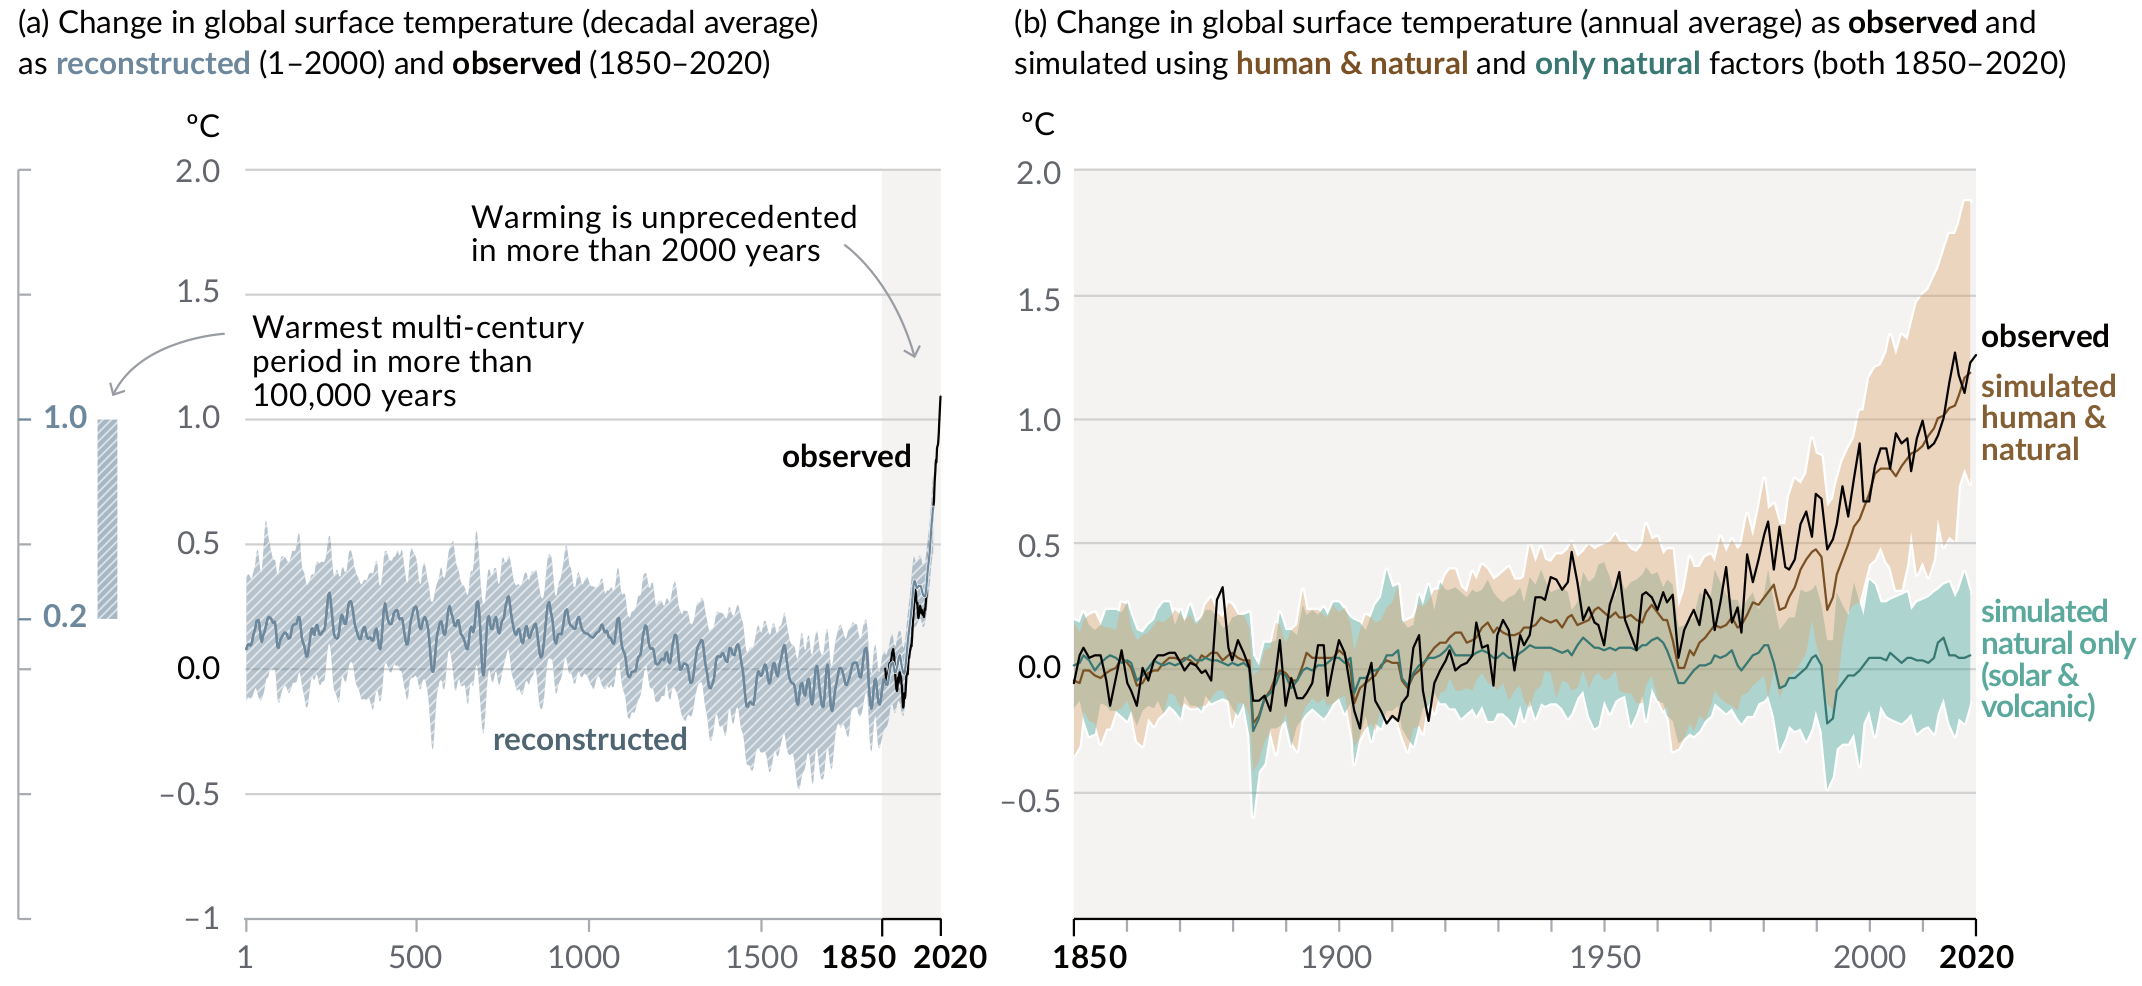
\includegraphics[width=1.0\textwidth]{plots/WG1_temperature.png}
      \end{center}   
    \end{columns}

  \end{scriptsize}
  \end{frame}  


%%%%%%%%%%%%%%%%%%%%%%%%%%%%%%%%%%%%%%%%%%%%%%%%%%%%%%%%%%%%%%%%%%%%%%%%%%%%%%%%%%
\begin{frame}
  \frametitle{\centerline{\hhref{https://www.ipcc.ch/report/ar6/wg1/downloads/report/IPCC_AR6_WGI_SPM_final.pdf}{IPCC Physical Science Basis:} Five illustrative scenarios for future CO$_2$ emissions}}
  \begin{scriptsize}

    \begin{columns}
      \column{0.4\textwidth}
      \begin{itemize}\setlength\itemsep{2.0ex}        
        \item[o] Illustrative scenarios for five possible socio-economic pathways starting in 2015, with their corresponding anthropogenic CO$_2$ and other greenhouse gas (GHG) emissions. They are referred to as the Shared Socio-economic Pathways and they are labelled as SSPx-y, with x ranging from 1 to 5, and y referring to the approximate level of radiative forcing (in watts per square metre).

        \item[o] {\cb SSP3-7.0 and SSP5-8.5} are scenarios with high and very high greenhouse gas emissions that roughly double from current levels by 2100 and 2050, respectively. 
        
        \item[o] {\cb SSP2-4.5} is a scenario with these emissions remaining around current levels until the middle of the century, then starting to decline. 
        
        \item[o] {\cb SSP1-1.9 and SSP1-2.6} are scenarios with very low and low emissions, declining to net zero around 2050, followed by varying levels of net negative CO$_2$ emissions due to anthropogenic removals of CO$_2$.
    \end{itemize}

      \column{0.6\textwidth}
      \begin{center}
          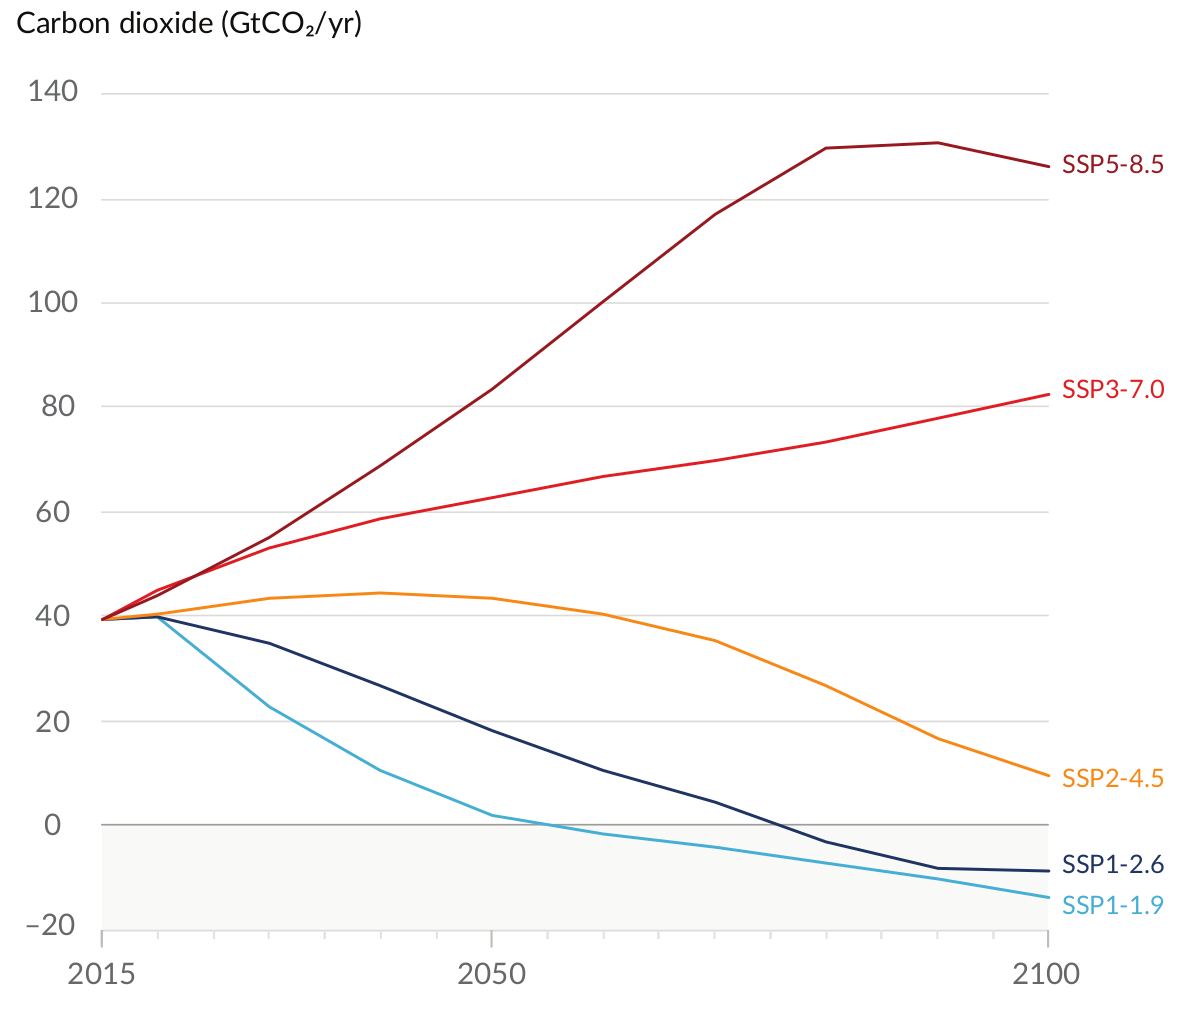
\includegraphics[width=1.0\textwidth]{plots/WG1_co2_scenarios.png}
      \end{center}   
    \end{columns}

  \end{scriptsize}
  \end{frame}

  %%%%%%%%%%%%%%%%%%%%%%%%%%%%%%%%%%%%%%%%%%%%%%%%%%%%%%%%%%%%%%%%%%%%%%%%%%%%%%%%%%
\begin{frame}
  \frametitle{\centerline{\hhref{https://www.ipcc.ch/report/ar6/wg1/downloads/report/IPCC_AR6_WGI_SPM_final.pdf}{IPCC Physical Science Basis:} Predicted temperature for five CO$_2$ scenarios}}
  \begin{scriptsize}

    \begin{columns}
      \column{0.34\textwidth}
      \begin{itemize}\setlength\itemsep{2.9ex}
      \item[o] {\bf Global surface temperature will continue to increase until at least mid-century under all considered emissions scenarios.} 
 
      \item[o] Global warming of 1.5$^\circ$C and 2$^\circ$C will be exceeded during the 21st century, unless deep reductions in CO$_2$ and other greenhouse gas emissions occur in the coming decades.

      \item[o] Extreme weather, rising seas and damaged ecosystems could threaten the safety and livelihoods of billions of people. 

      \item[o] {\it There could be 1.2 billion climate refugees by 2050} - \hhref{https://www.zurich.com/en/media/magazine/2022/there-could-be-1-2-billion-climate-refugees-by-2050-here-s-what-you-need-to-know}{Ecological Threat Register}

      \end{itemize}

      \column{0.7\textwidth}
      \begin{center}
          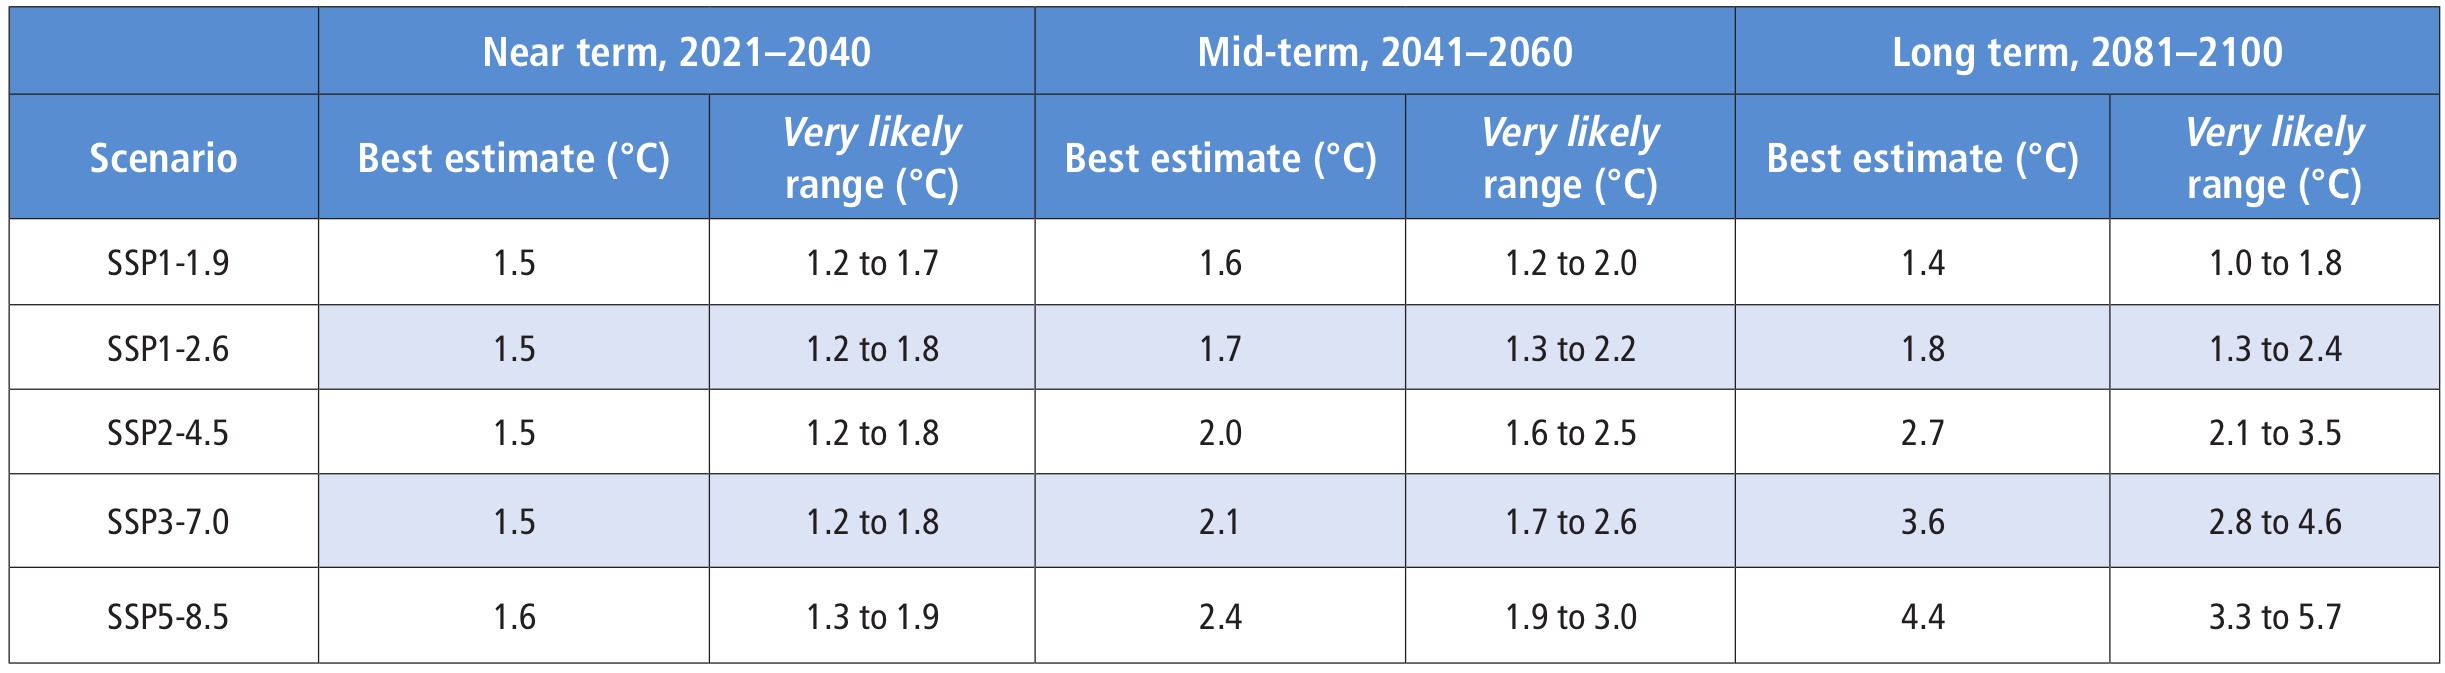
\includegraphics[width=1.0\textwidth]{plots/WG1_predicted_temperature_table.png}\\
          \vspace{0.2cm}
          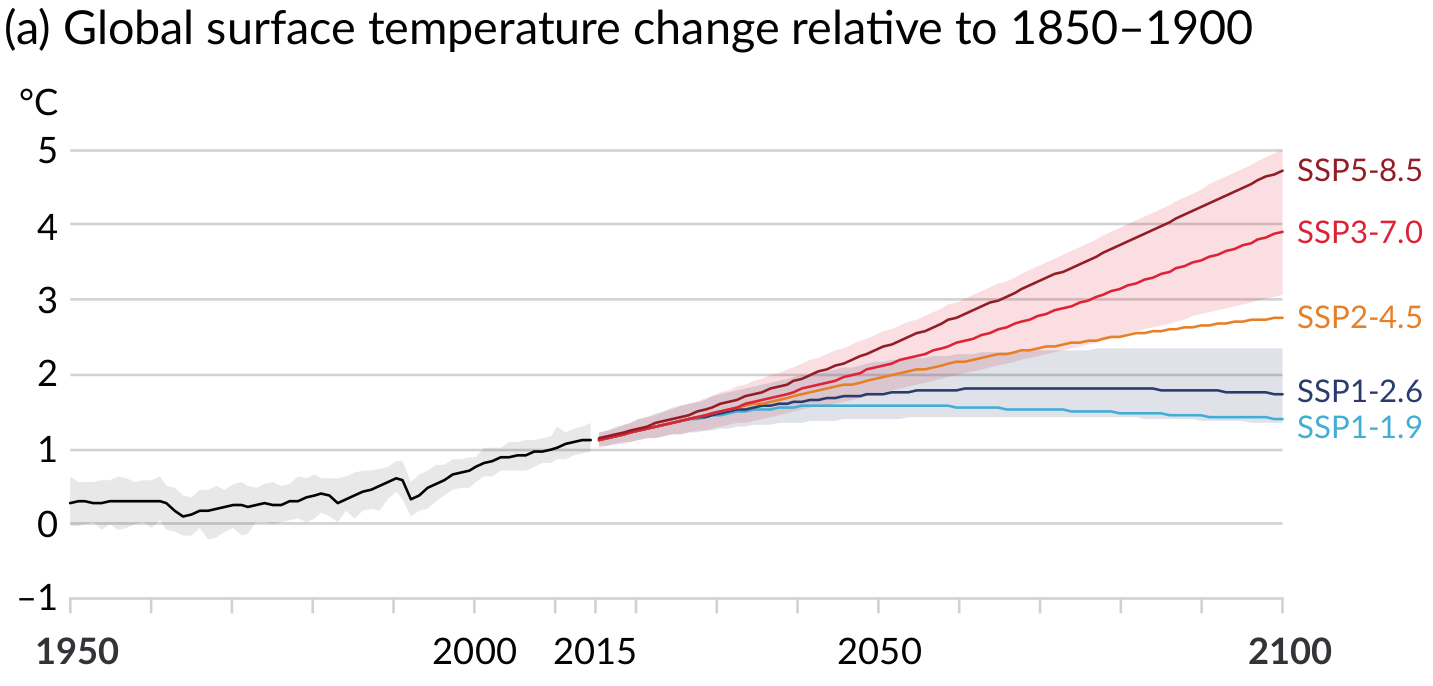
\includegraphics[width=1.0\textwidth]{plots/WG1_SSPs_surface_temperature.png}
      \end{center}   
    \end{columns}

  \end{scriptsize}
  \end{frame}  

%%%%%%%%%%%%%%%%%%%%%%%%%%%%%%%%%%%%%%%%%%%%%%%%%%%%%%%%%%%%%%%%%%%%%%%%%%%%%%%%%%
\begin{frame}
\frametitle{\centerline{\hhref{https://www.ipcc.ch/report/ar6/wg1/downloads/report/IPCC_AR6_WGI_SPM_final.pdf}{IPCC Physical Science Basis:} Predicted surface temperature maps for five CO$_2$ scenarios}}
\begin{scriptsize}

  \begin{columns}

    \column{0.85\textwidth}
    \begin{center}
        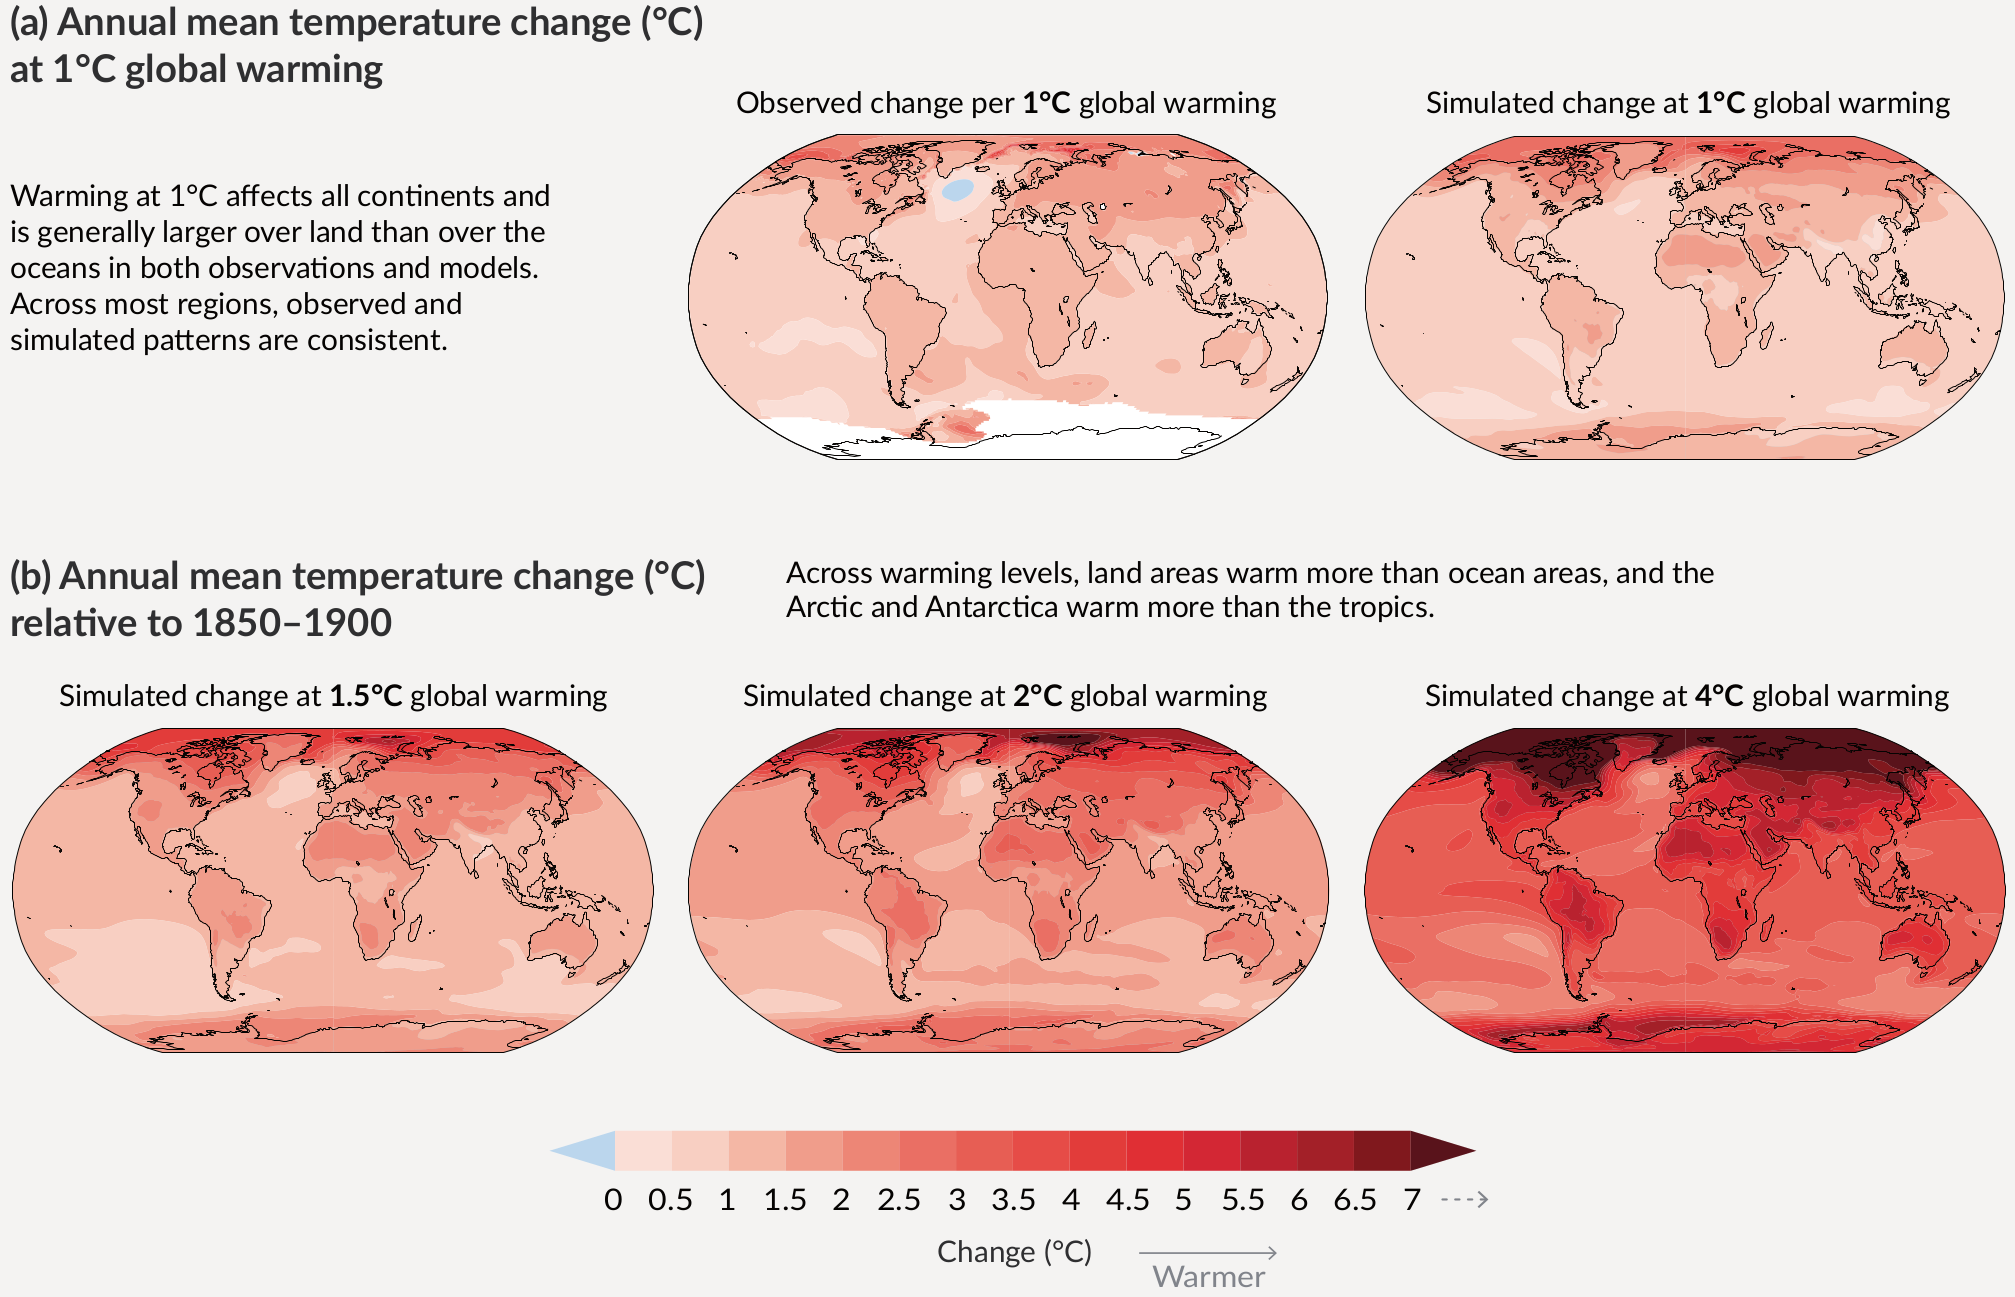
\includegraphics[width=1.0\textwidth]{plots/WG1_SSPs_surface_temperature_maps}
    \end{center}   
  \end{columns}

\end{scriptsize}
\end{frame}  


  %%%%%%%%%%%%%%%%%%%%%%%%%%%%%%%%%%%%%%%%%%%%%%%%%%%%%%%%%%%%%%%%%%%%%%%%%%%%%%%%%%
  \begin{frame}
    \frametitle{\centerline{\hhref{https://www.ipcc.ch/report/ar6/wg1/downloads/report/IPCC_AR6_WGI_SPM_final.pdf}{IPCC Physical Science Basis:} Predicted sea ice melting and sea level raise}}
    \begin{scriptsize}
  
      \begin{columns}
        \column{1.0\textwidth}
        \begin{itemize}\setlength\itemsep{1.9ex}        
          \item[o] {\cb Left:} Past greenhouse gas and CO$_2$ emissions since 1750 have committed the global ocean to future warming (high confidence). Mountain and polar glaciers are committed to continue to melt for decades or centuries (very high confidence). {\it Loss of permafrost carbon following permafrost thaw is irreversible at centennial time scales (high confidence).} Continued ice loss over the 21st century is virtually certain for the Greenland ice sheet and likely for the Antarctic ice sheet. 
  
          \item[o] {\cb Right:} It is virtually certain that global mean sea level will continue to rise over the 21st century. Relative to 1995-2014, the likely global mean sea level rise by 2100 is 0.28-0.55~meter even under the very low GHG emissions scenario (SSP1-1.9), and is 0.32-0.62~meter under the low GHG emissions scenario (SSP1-2.6). Global mean sea level rise of about 2~meter by 2100 and 5~meter by 2150 under a very high GHG emissions scenario (SSP5-8.5) (low confidence) cannot be ruled out due to deep uncertainty in ice-sheet processes.
      \end{itemize}
  
      \end{columns}

      \begin{columns}
        \column{0.5\textwidth}
        \begin{center}
            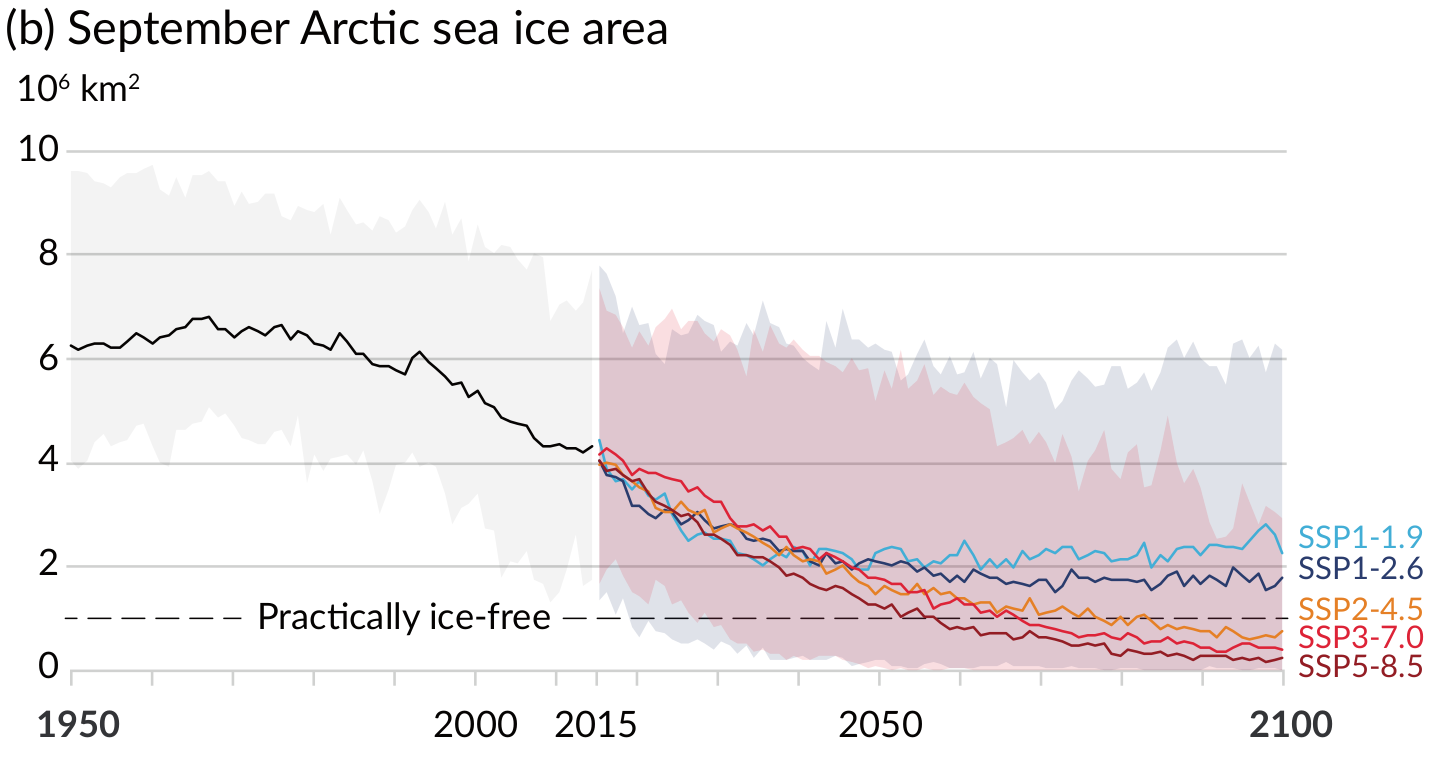
\includegraphics[width=1.0\textwidth]{plots/WG1_SSPs_artic_icearea.png.png}
        \end{center}   

        \column{0.5\textwidth}
        \begin{center}
            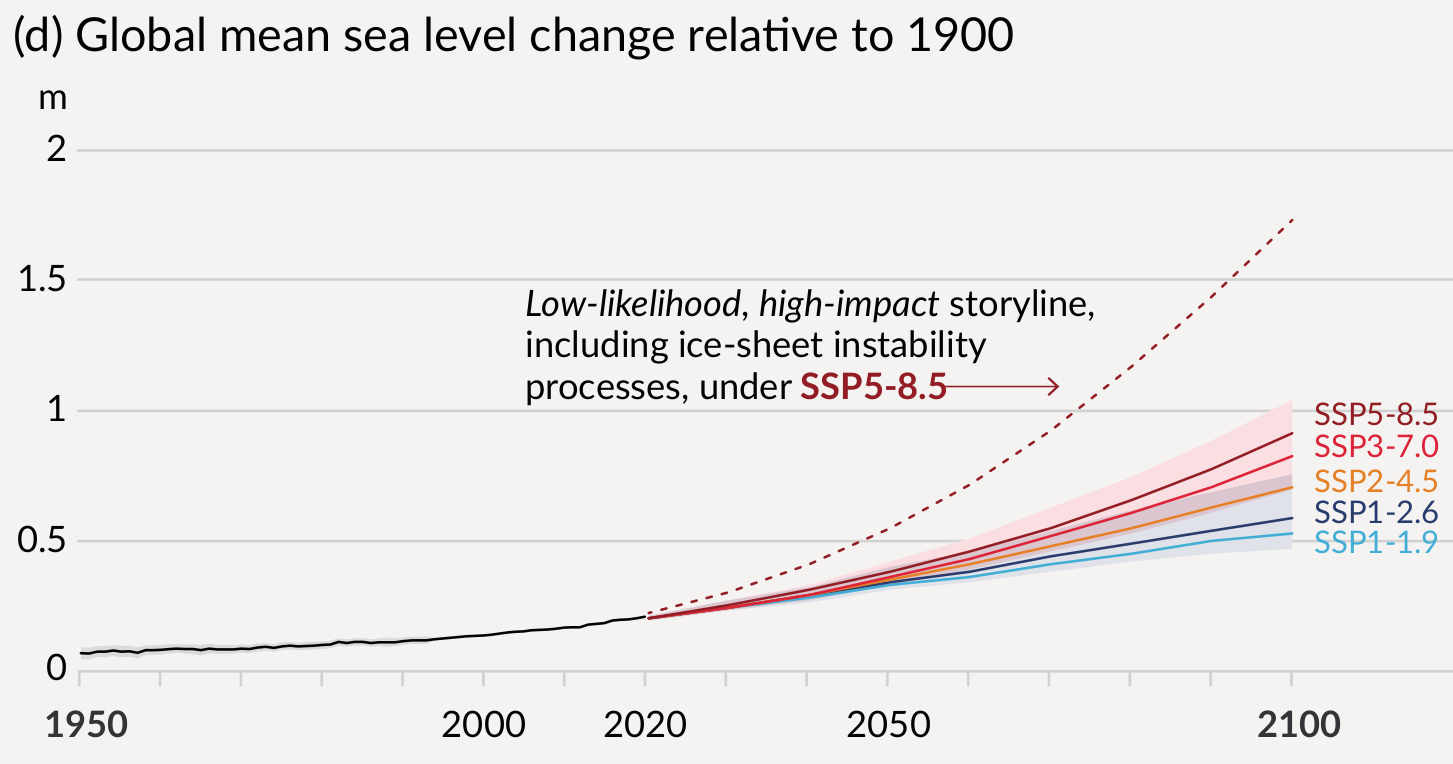
\includegraphics[width=1.0\textwidth]{plots/WG1_SSPs_sea_level_change.png}
        \end{center}   
      \end{columns}
  
    \end{scriptsize}
    \end{frame}  

%%%%%%%%%%%%%%%%%%%%%%%%%%%%%%%%%%%%%%%%%%%%%%%%%%%%%%%%%%%%%%%%%%%%%%%%%%%%%%%%%%
%%%%%%%%%%%%%%%%%%%%%%%%%%%%%%%%%%%%%%%%%%%%%%%%%%%%%%%%%%%%%%%%%%%%%%%%%%%%%%%%%%


%%%%%%%%%%%%%%%%%%%%%%%%%%%%%%%%%%%%%%%%%%%%%%%%%%%%%%%%%%%%%%%%%%%%%%%%%%%%%%%%%%
%%%%%%%%%%%%%%%%%%%%%%%%%%%%%%%%%%%%%%%%%%%%%%%%%%%%%%%%%%%%%%%%%%%%%%%%%%%%%%%%%%
\begin{frame}
  \begin{small}
              
  \begin{columns}
  \column{0.9\textwidth}
    \hhref{https://wir2022.wid.world/download}{World Inequality Report 2022}
    \begin{itemize}\setlength\itemsep{1.0ex}\footnotesize
      \item[o] Beautifully presented data on regional and societal inequalities in income, wealth, and carbon emissions
    \end{itemize}
  \end{columns}

  \end{small}
  \end{frame}

%%%%%%%%%%%%%%%%%%%%%%%%%%%%%%%%%%%%%%%%%%%%%%%%%%%%%%%%%%%%%%%%%%%%%%%%%%%%%%%%%%
\begin{frame}
  \frametitle{\centerline{ \hhref{https://wir2022.wid.world/download/}{World Inequality Report:} Total CO$_2$ emissions per region}}
  \begin{scriptsize}

    \begin{columns}
      \column{1.0\textwidth}
      \begin{itemize}\setlength\itemsep{1.3ex}        
        \item[o] {\cb Left:} This graph shows the breakdown of the global CO$_2$ emissions by major economic regions as a function of time. Total global CO$_2$ emissions in 2019 were 50 billion tonnes. After 1990, emissions include carbon and other greenhouse gases embedded in imports/exports of goods and services from/to other regions. {\it Close to half (46\%) of historical CO$_2$ emissions were released after 1990.}

        \item[o] {\cb Right:} The graph shows historical emissions by region (left bar) and the remaining global carbon budget (centre and right bars) to have 83\% chances to stay under 1.5°C and 2°C, according to IPCC Assessment Report 6 (2021). Regional emissions are net of carbon embedded in imports of goods and services from other regions.
    \end{itemize}

    \end{columns}

    \vspace{0.4cm}
    \begin{columns}
      \column{0.6\textwidth}
      \begin{center}
          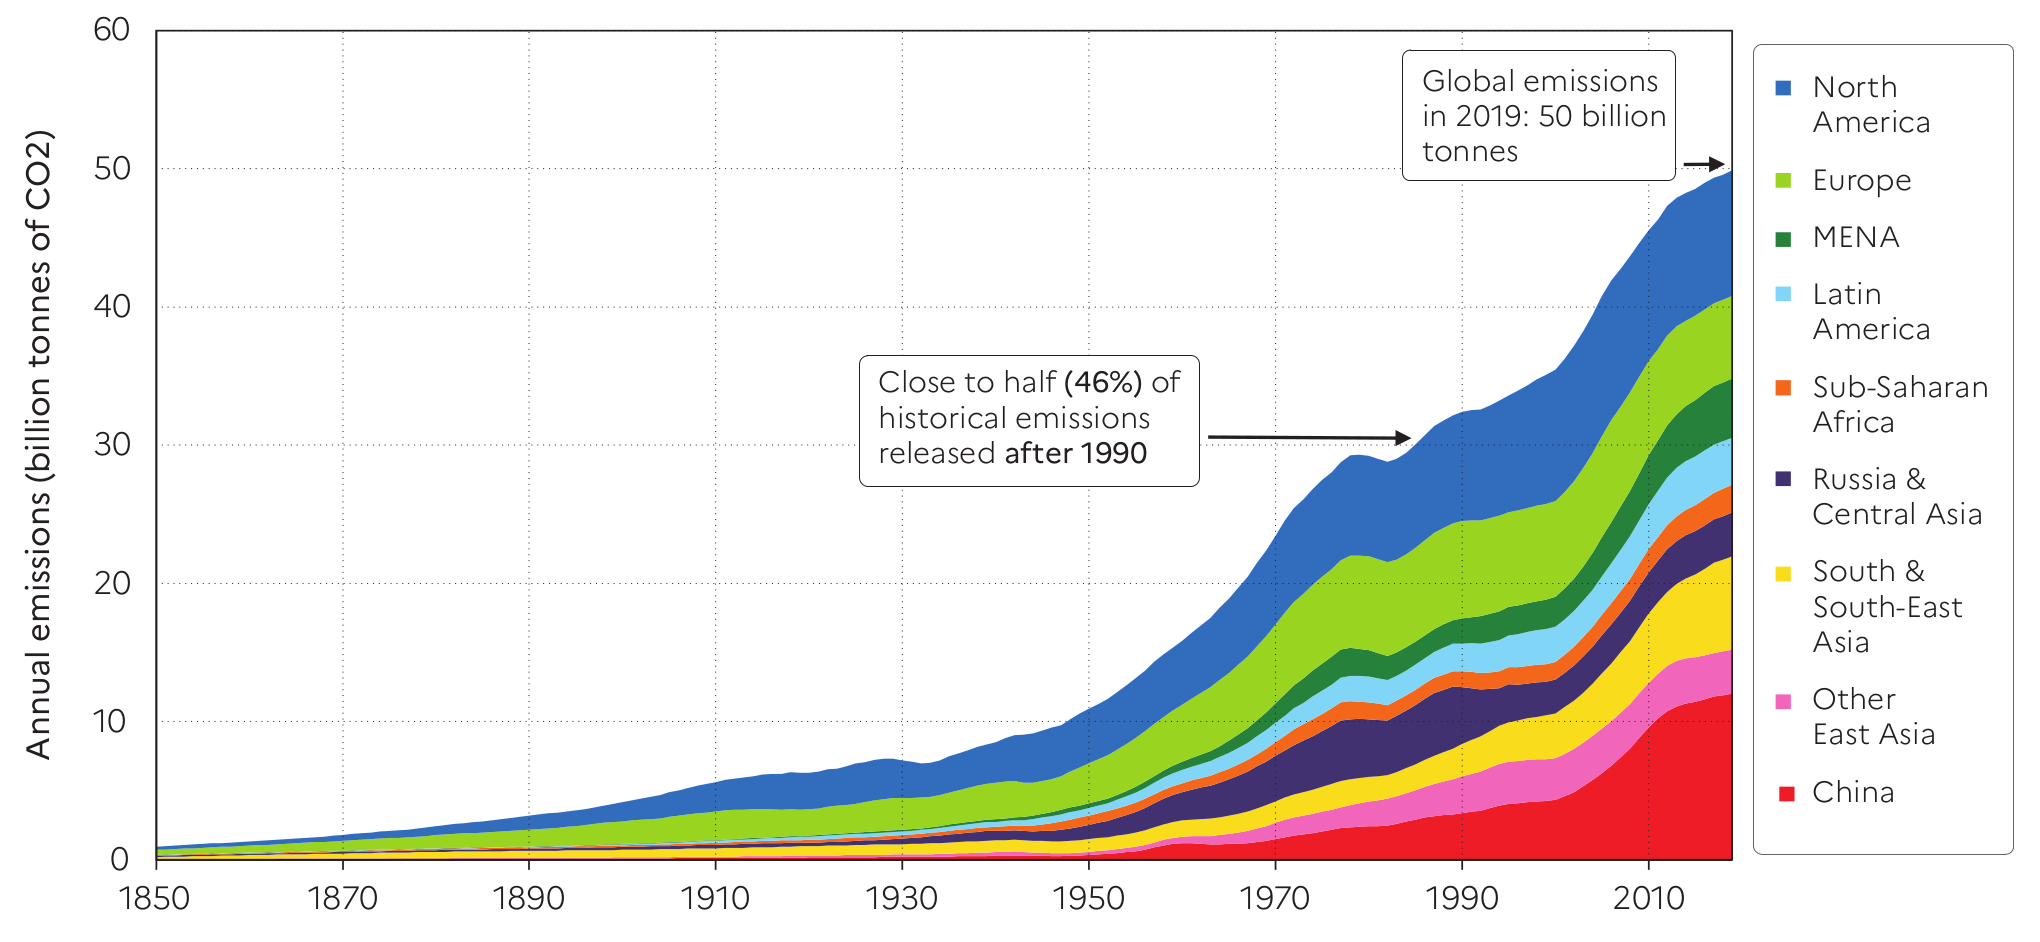
\includegraphics[width=1.0\textwidth]{plots/WIR_co2_per_region_vs_time}
      \end{center}

      \column{0.5\textwidth}
      \begin{center}
        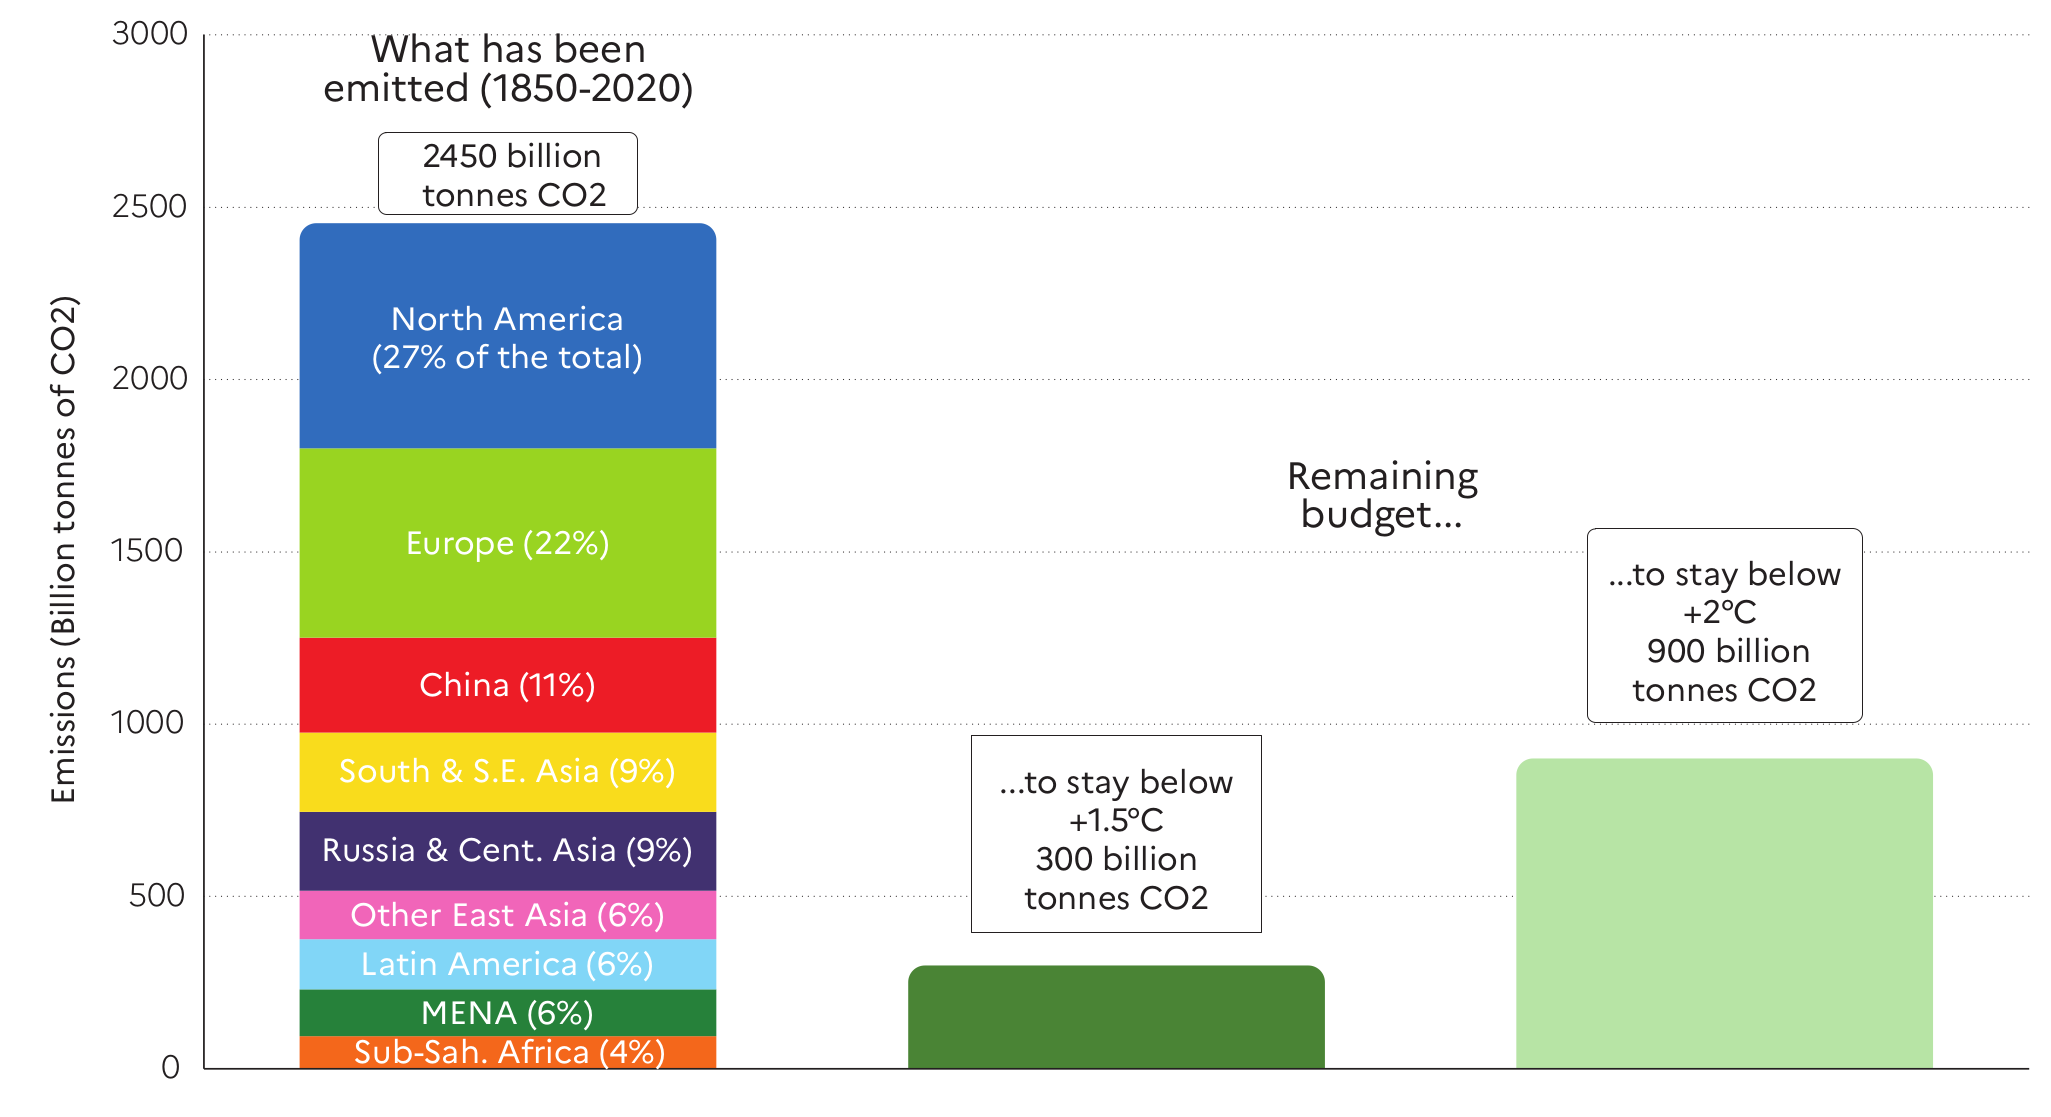
\includegraphics[width=1.0\textwidth]{plots/WIR_budget_emitted_and_allowed}
      \end{center}      
    \end{columns}

  \end{scriptsize}
  \end{frame}  

%%%%%%%%%%%%%%%%%%%%%%%%%%%%%%%%%%%%%%%%%%%%%%%%%%%%%%%%%%%%%%%%%%%%%%%%%%%%%%%%%%
\begin{frame}
  \frametitle{\centerline{ \hhref{https://wir2022.wid.world/download/}{World Inequality Report:} Average per capita CO$_2$ emissions in 2019}}
  \begin{scriptsize}

    \begin{columns}
      \column{1.0\textwidth}
      \begin{itemize}\setlength\itemsep{1.3ex}        
        \item[o] {\cb Left:} CO2 emissions in tonnes per capita, per year for different regions. The world average is 6.6 tons per capita. This needs to go down to 3.4 tons in order to limit global warming to 2 degrees above the pre-industrial level.

        \item[o] {\cb Right:} {\it The top 10\% of emitters are responsible for close to 50\% of all emissions, while the bottom 50\% produce 12\% of the total.}

        \item[o] Personal carbon footprints include emissions from domestic consumption, public and private investments as well as imports and exports of carbon embedded in goods and services traded with the rest of the world.
    \end{itemize}
    \end{columns}

    \vspace{0.4cm}
    \begin{columns}      
      \column{0.4\textwidth}
      \begin{center}
          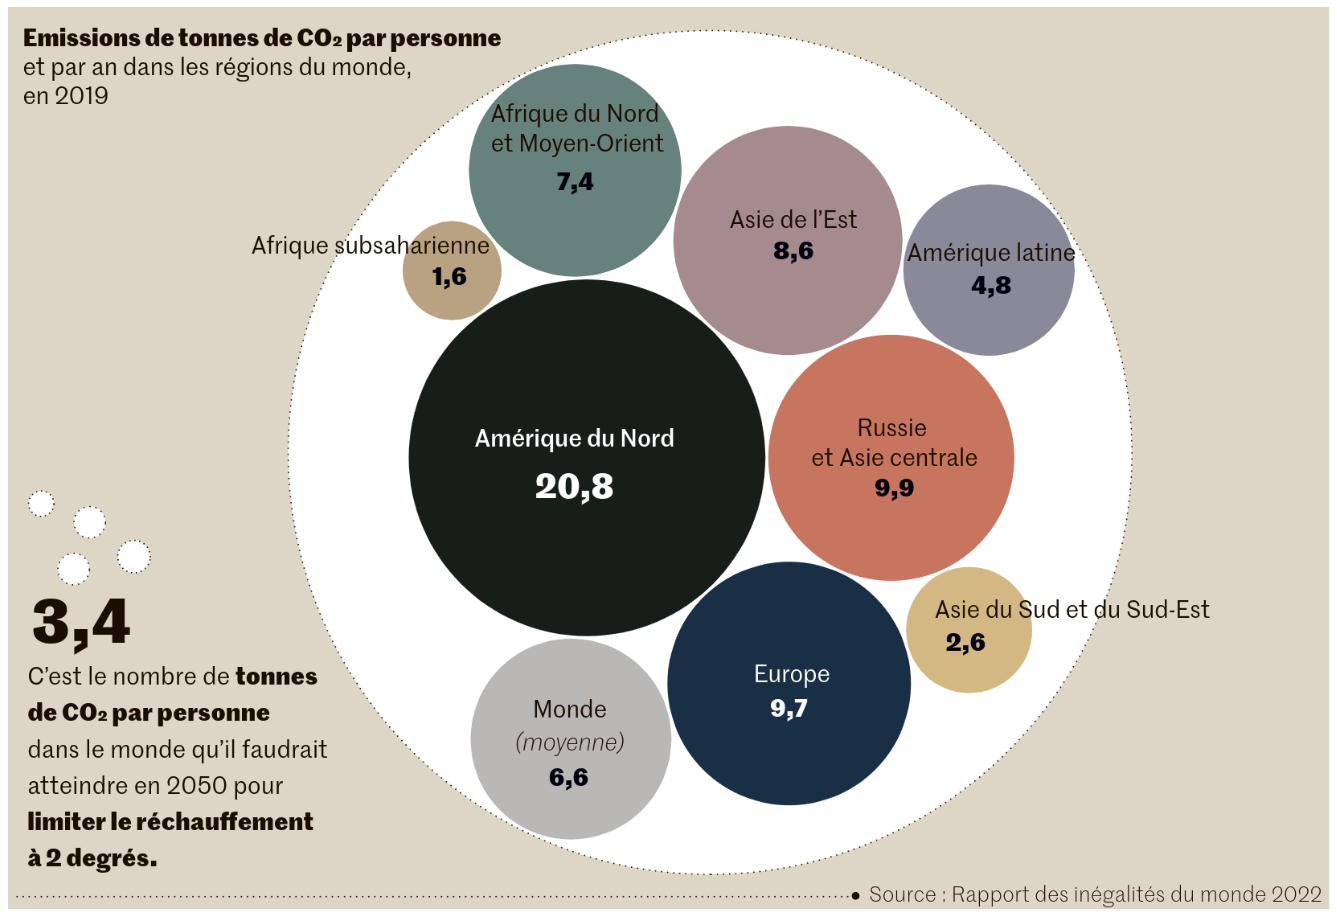
\includegraphics[width=1.0\textwidth]{plots/co2.png}
      \end{center}  

      \column{0.6\textwidth}
      \begin{center}
          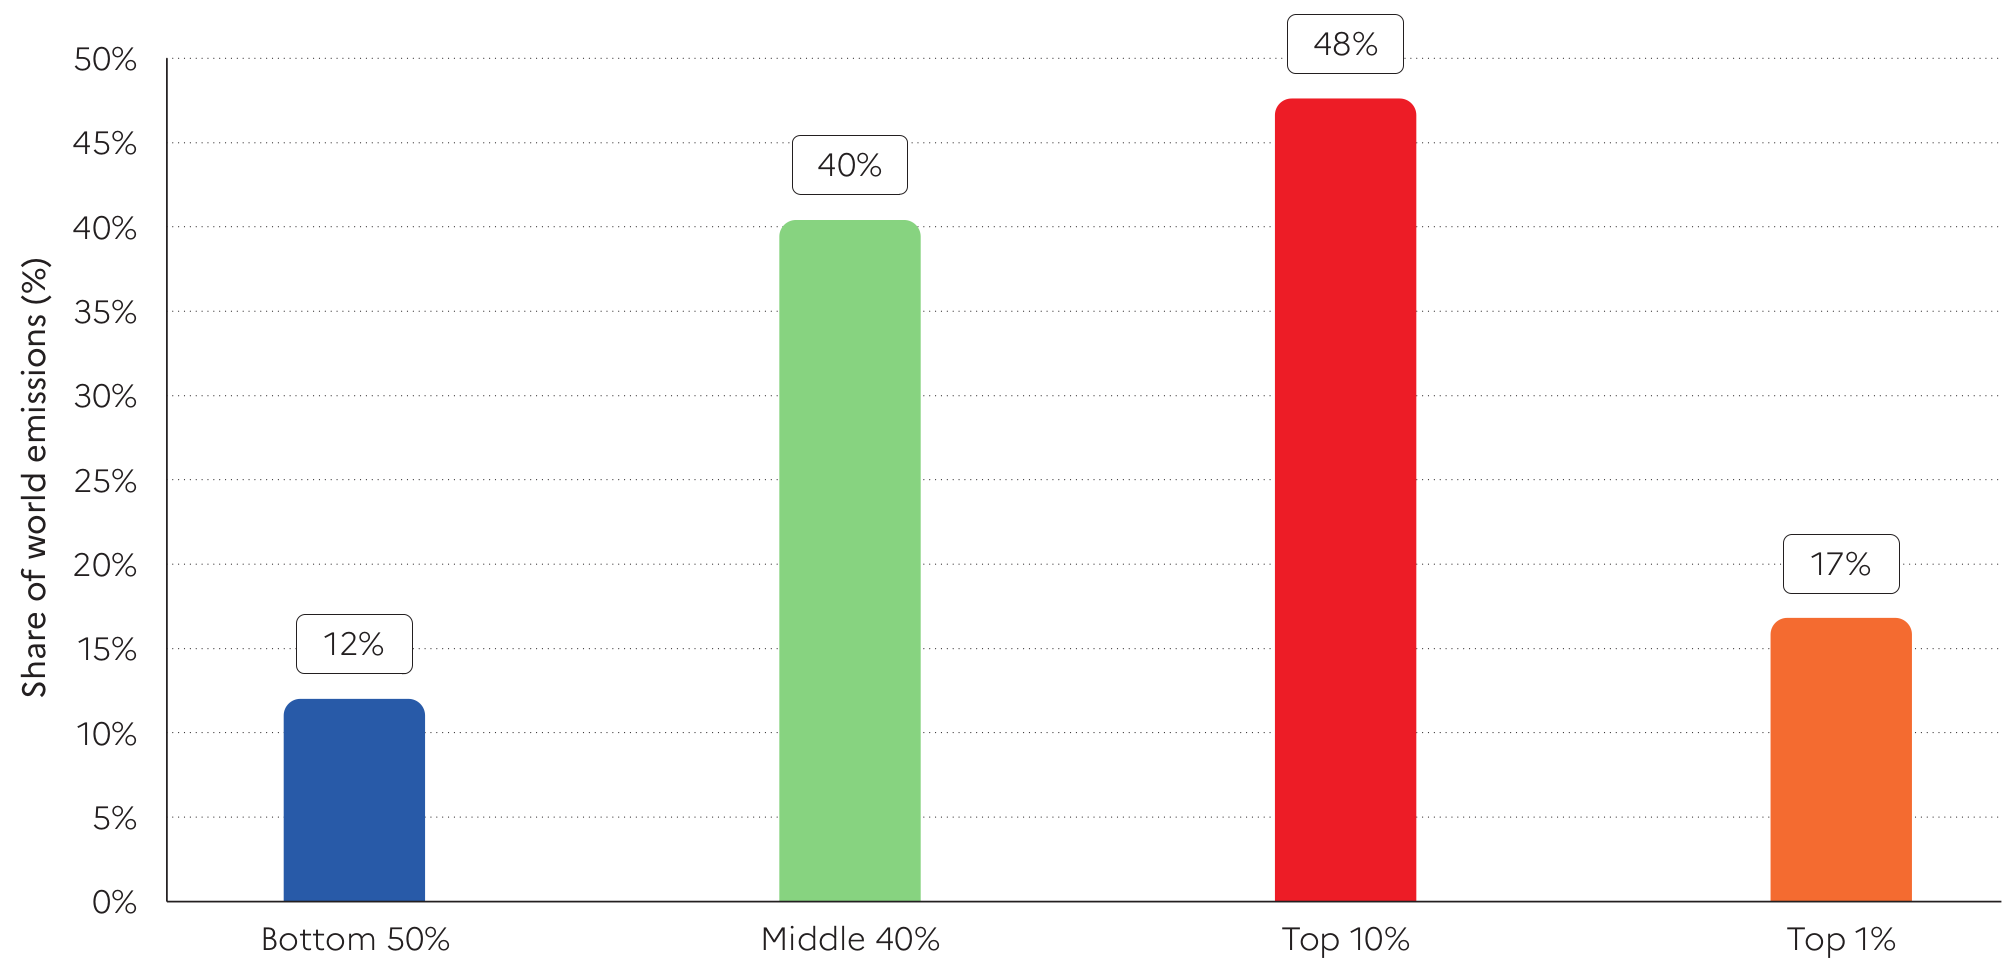
\includegraphics[width=1.0\textwidth]{plots/WIR_budget.png}
      \end{center}
    \end{columns}

  \end{scriptsize}
  \end{frame}  

%%%%%%%%%%%%%%%%%%%%%%%%%%%%%%%%%%%%%%%%%%%%%%%%%%%%%%%%%%%%%%%%%%%%%%%%%%%%%%%%%%
\begin{frame}
  \frametitle{\centerline{ \hhref{https://wir2022.wid.world/download/}{World Inequality Report:} Breakdown of per capita CO$_2$ emissions}}
  \begin{scriptsize}

    \begin{columns}
      \column{1.0\textwidth}
      \begin{itemize}\setlength\itemsep{1.3ex}        
        \item[o] CO$_2$ emissions of bottom 50\% of emitters per capita per year: 5 tonnes in Europe, 13 tonnes in East Asia, 10 tonnes in North America.

        \item[o] CO$_2$ emissions of top 10\% of emitters per capita per year: 29 tonnes in Europe, 39 tonnes in East Asia, 73 tonnes in North America.

        \item[o] Poorest half of the population in rich countries is already at (or near) the 2030 climate per-capita targets set by rich countries. This is not the case for the top half of the population. Large inequalities in emissions suggest that climate policies should target wealthy polluters more. So far, climate policies such as carbon taxes have often disproportionately impacted low and middle-income groups, while leaving the consumption habits of wealthiest groups unchanged.
    \end{itemize}
    \end{columns}

    \begin{columns}
      \column{0.5\textwidth}
      \begin{center}
          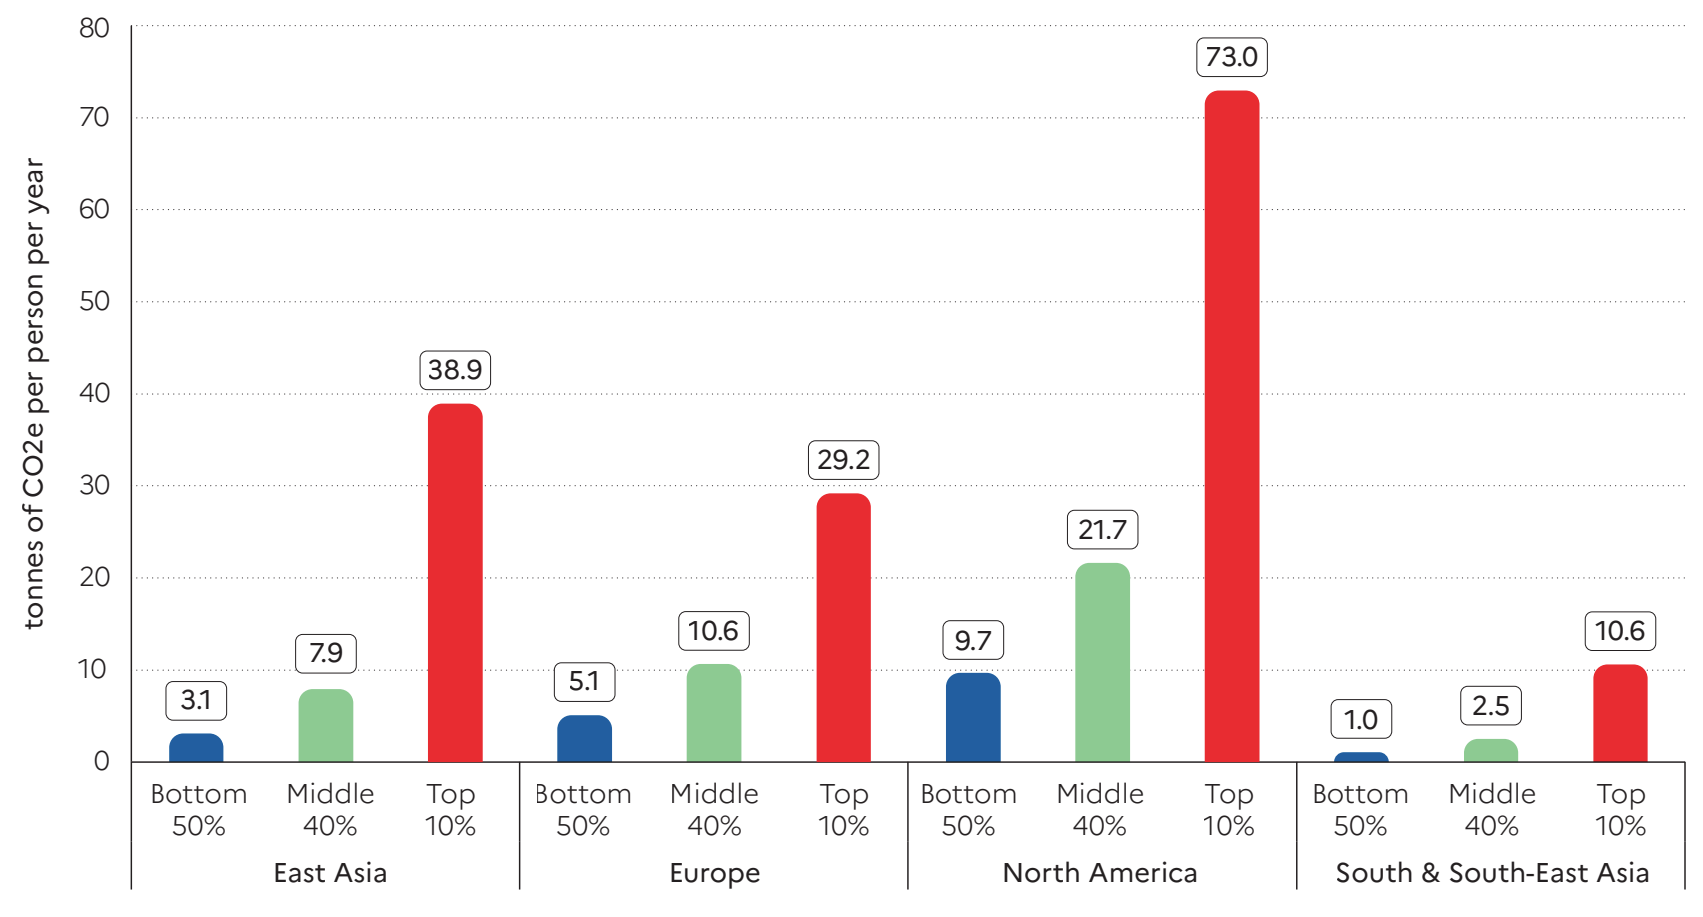
\includegraphics[width=1.0\textwidth]{plots/WIR_carbon_per_capita_west.png}
      \end{center}

      \column{0.5\textwidth}
      \begin{center}
        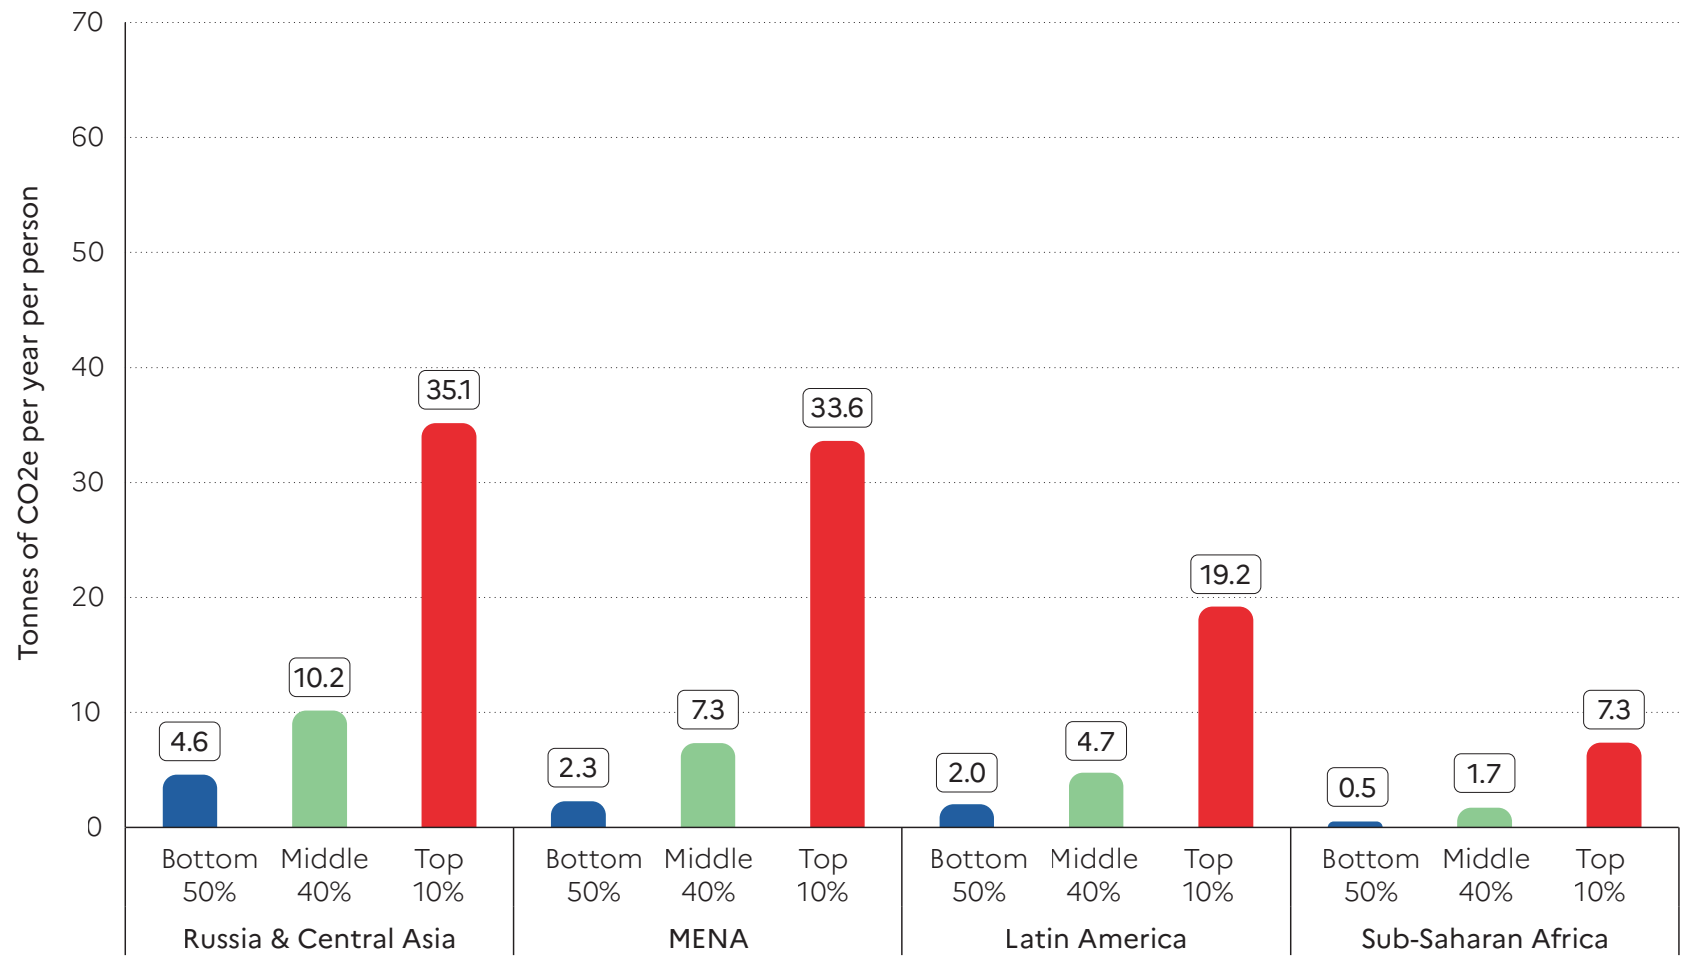
\includegraphics[width=1.0\textwidth]{plots/WIR_carbon_per_capita_rest.png}
      \end{center}      
    \end{columns}

  \end{scriptsize}
  \end{frame}

%%%%%%%%%%%%%%%%%%%%%%%%%%%%%%%%%%%%%%%%%%%%%%%%%%%%%%%%%%%%%%%%%%%%%%%%%%
%%%%%%%%%%%%%%%%%%%%%%%%%%%%%%%%%%%%%%%%%%%%%%%%%%%%%%%%%%%%%%%%%%%%%%%%%%


%%%%%%%%%%%%%%%%%%%%%%%%%%%%%%%%%%%%%%%%%%%%%%%%%%%%%%%%%%%%%%%%%%%%%%%%%%
%%%%%%%%%%%%%%%%%%%%%%%%%%%%%%%%%%%%%%%%%%%%%%%%%%%%%%%%%%%%%%%%%%%%%%%%%%
\begin{frame}
  \begin{small}
              
  \begin{columns}
  \column{0.9\textwidth}
  {\cb Intergovernmental Panel on Climate Change (IPCC) Assessment Report 6 (2021)}
    \begin{itemize}\setlength\itemsep{1.0ex}\footnotesize
      \item[1.]  \hhref{https://report.ipcc.ch/ar6wg2/pdf/IPCC_AR6_WGII_SummaryForPolicymakers.pdf}{Working Group II: Impacts, Adaptation and Vulnerability}
    \end{itemize}
  \end{columns}

  \end{small}
\end{frame}  

%%%%%%%%%%%%%%%%%%%%%%%%%%%%%%%%%%%%%%%%%%%%%%%%%%%%%%%%%%%%%%%%%%%%%%%%%%%%%%%%%%
\begin{frame}
  \frametitle{\centerline{\hhref{https://report.ipcc.ch/ar6wg2/pdf/IPCC_AR6_WGII_SummaryForPolicymakers.pdf}{IPCC Impacts, Adaptation and Vulnerability:} Climate change impact on natural ecosystems}}
  \begin{scriptsize}

    \begin{columns}
      \column{1.0\textwidth}
      \begin{itemize}\setlength\itemsep{1.9ex}        
        \item[o] A
      \end{itemize}

    \end{columns}

    \vspace{-0.1cm}
    \begin{columns}
      \column{0.9\textwidth}
      \begin{center}
          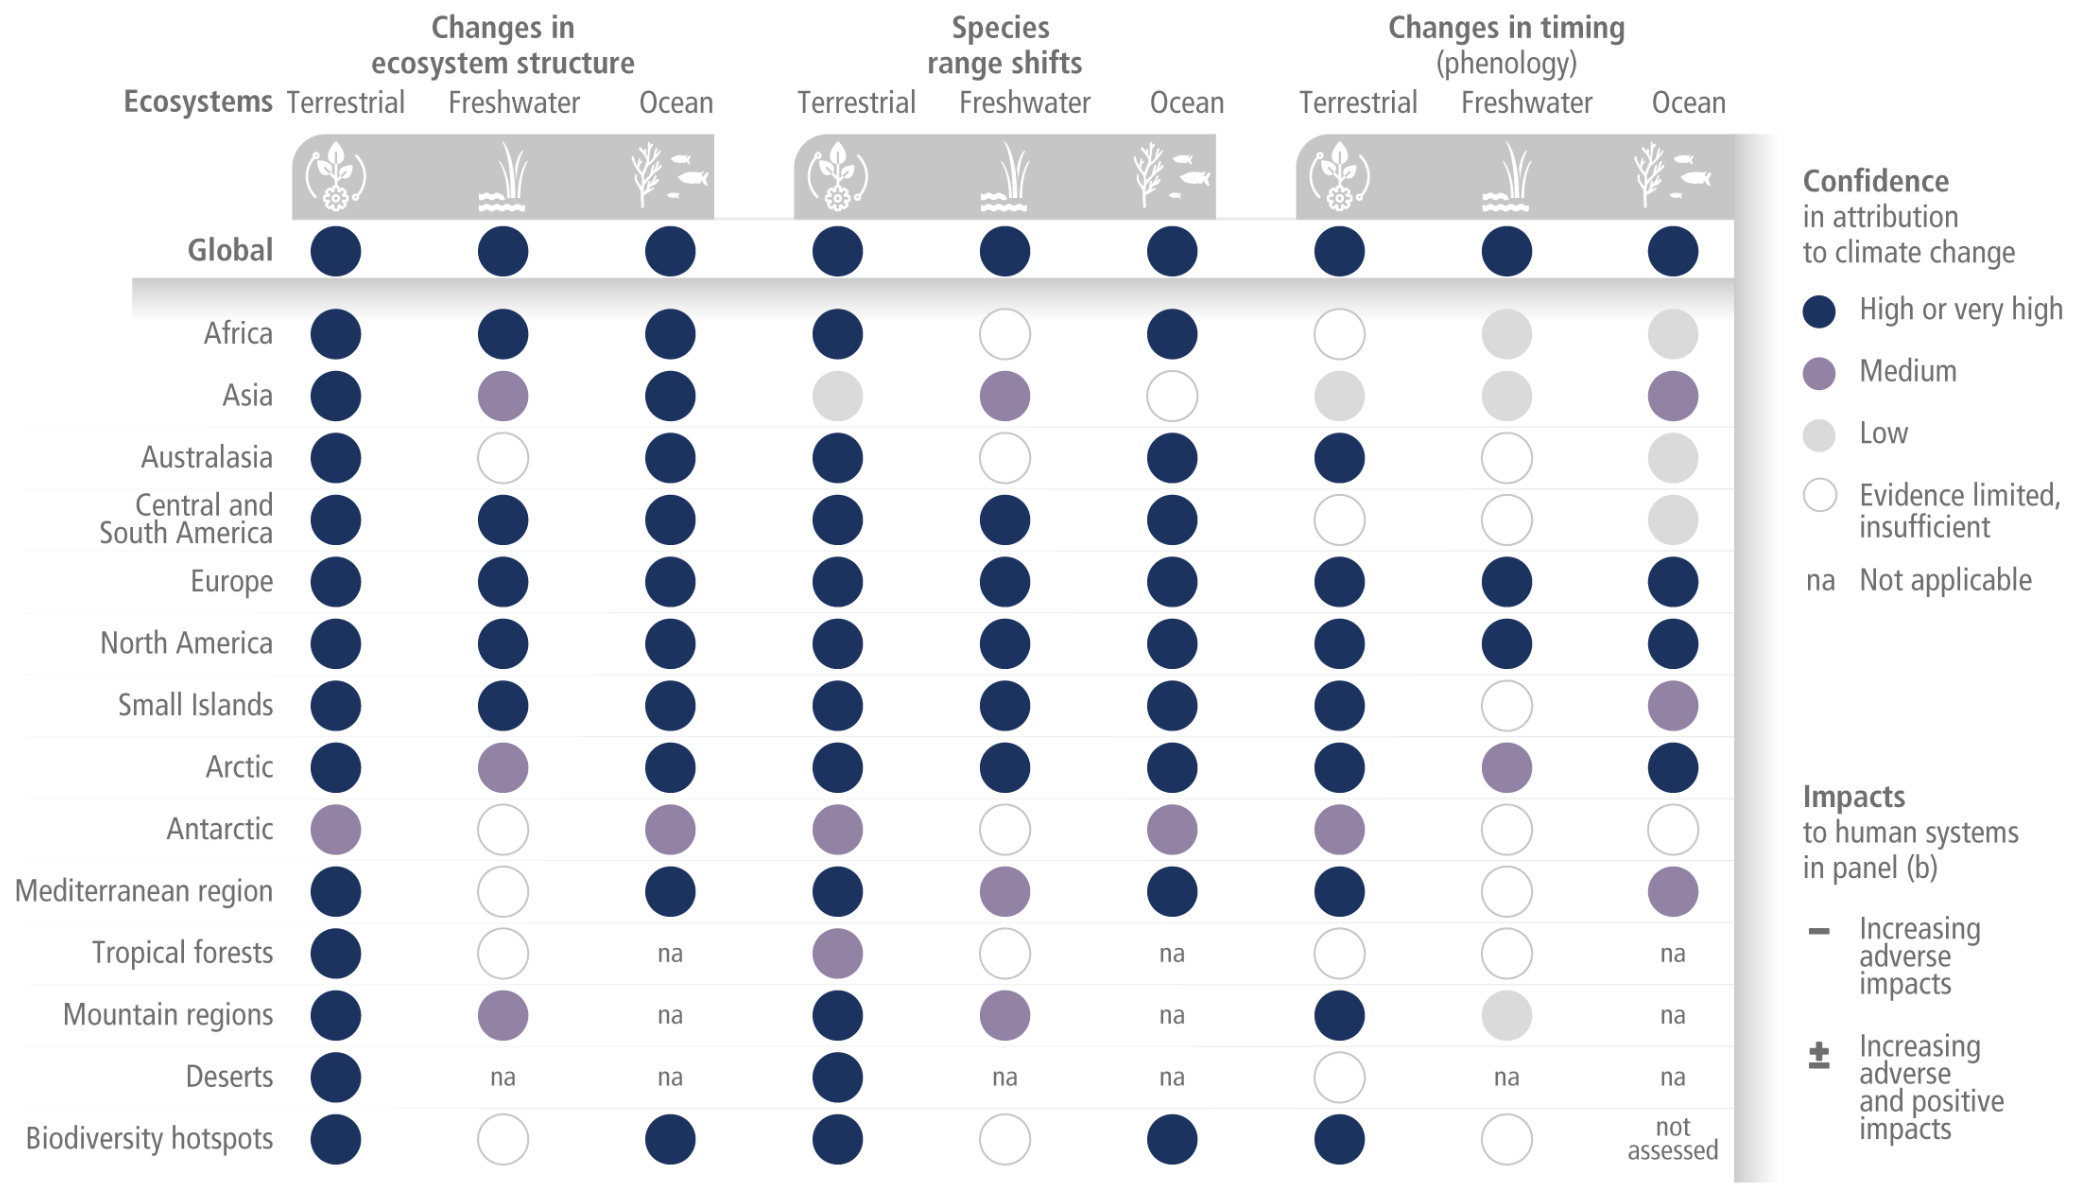
\includegraphics[width=1.0\textwidth]{plots/WG2_impact_on_ecosystems.png}
      \end{center}   
    \end{columns}

  \end{scriptsize}
  \end{frame}  

%%%%%%%%%%%%%%%%%%%%%%%%%%%%%%%%%%%%%%%%%%%%%%%%%%%%%%%%%%%%%%%%%%%%%%%%%%%%%%%%%%
\begin{frame}
  \frametitle{\centerline{\hhref{https://report.ipcc.ch/ar6wg2/pdf/IPCC_AR6_WGII_SummaryForPolicymakers.pdf}{IPCC Impacts, Adaptation and Vulnerability:} Climate change impact on human societies}}
  \begin{scriptsize}

    \begin{columns}
      \column{1.0\textwidth}
      \begin{itemize}\setlength\itemsep{1.9ex}        
        \item[o] B
      \end{itemize}

    \end{columns}

    \vspace{-0.1cm}
    \begin{columns}
      \column{0.9\textwidth}
      \begin{center}
          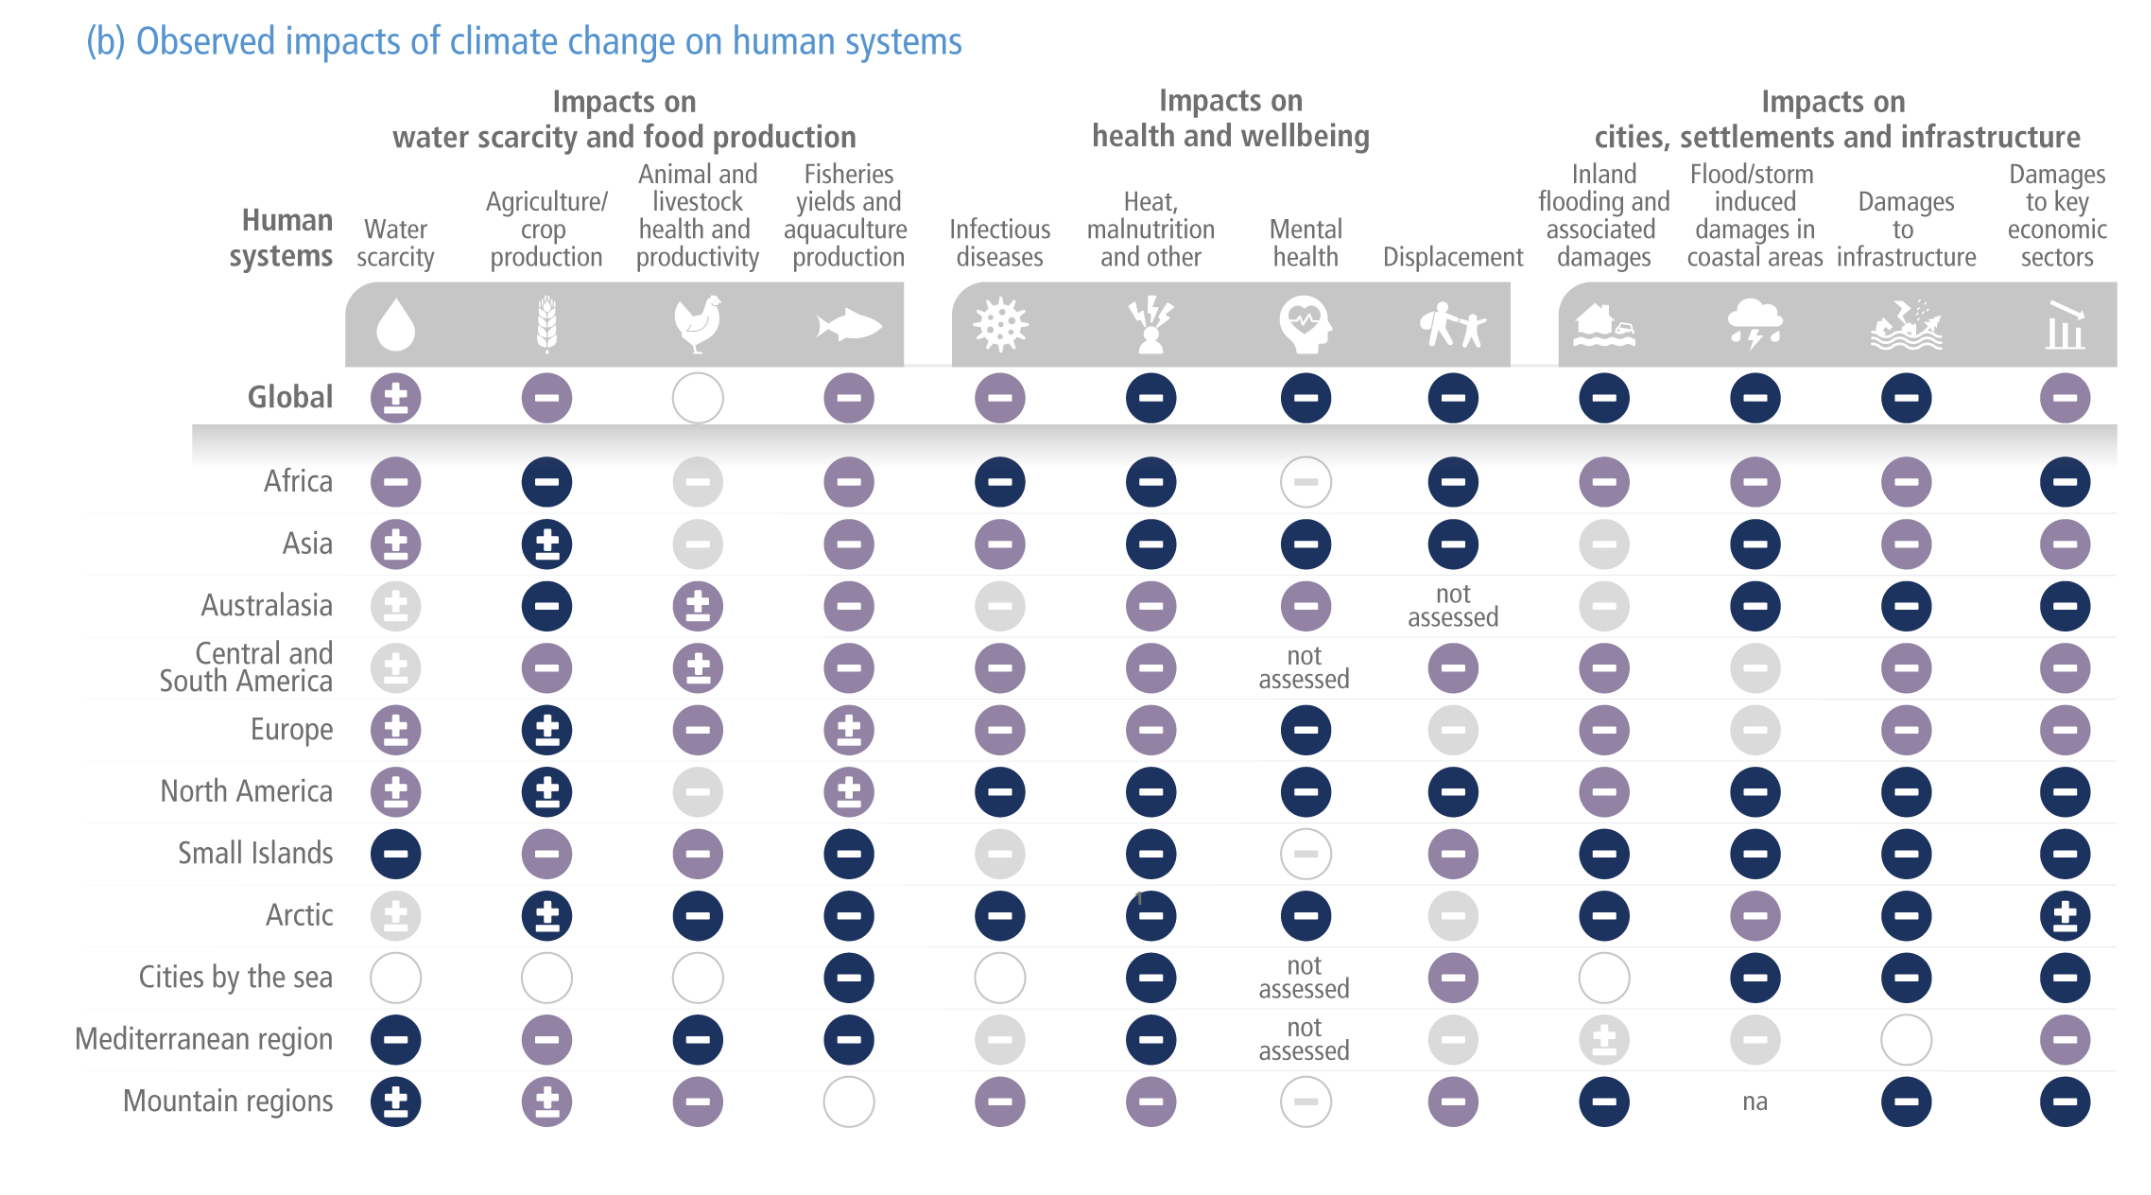
\includegraphics[width=1.0\textwidth]{plots/WG2_impact_on_society.png}
      \end{center}   
    \end{columns}

  \end{scriptsize}
  \end{frame}  

%%%%%%%%%%%%%%%%%%%%%%%%%%%%%%%%%%%%%%%%%%%%%%%%%%%%%%%%%%%%%%%%%%%%%%%%%%
%%%%%%%%%%%%%%%%%%%%%%%%%%%%%%%%%%%%%%%%%%%%%%%%%%%%%%%%%%%%%%%%%%%%%%%%%%


%%%%%%%%%%%%%%%%%%%%%%%%%%%%%%%%%%%%%%%%%%%%%%%%%%%%%%%%%%%%%%%%%%%%%%%%%%
%%%%%%%%%%%%%%%%%%%%%%%%%%%%%%%%%%%%%%%%%%%%%%%%%%%%%%%%%%%%%%%%%%%%%%%%%%
\begin{frame}
  \begin{small}
              
  \begin{columns}
  \column{0.9\textwidth}
  {\cb Intergovernmental Panel on Climate Change (IPCC) Assessment Report 6 (2021)}
    \begin{itemize}\setlength\itemsep{1.0ex}\footnotesize
      \item[1.]  \hhref{https://www.ipcc.ch/report/ar6/wg3/downloads/report/IPCC_AR6_WGIII_SPM.pdf}{Working Group III:  Mitigation of Climate Change}
    \end{itemize}
  \end{columns}

  \end{small}
\end{frame}  

%%%%%%%%%%%%%%%%%%%%%%%%%%%%%%%%%%%%%%%%%%%%%%%%%%%%%%%%%%%%%%%%%%%%%%%%%%%%%%%%%%
\begin{frame}
  \begin{scriptsize}

    \vspace{-0.1cm}
    \begin{columns}
      \column{0.43\textwidth}
      \begin{center}
          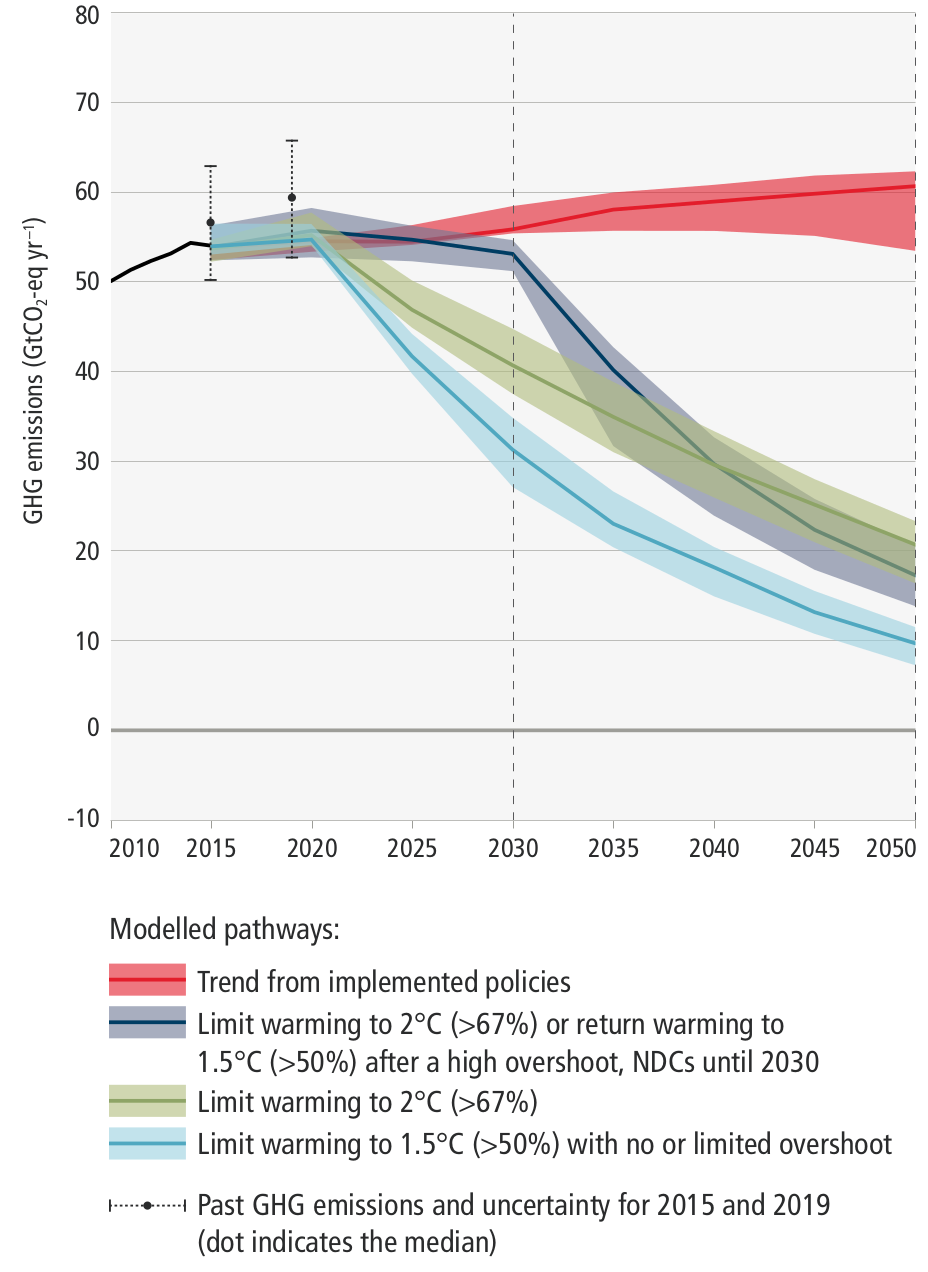
\includegraphics[width=1.0\textwidth]{plots/WG3_global_GHG_emissions.png}
      \end{center}  
      
      \column{0.5\textwidth}
      \begin{itemize}\setlength\itemsep{1.9ex}        
        \item[o] \hhref{https://www.ipcc.ch/report/ar6/wg3/downloads/report/IPCC_AR6_WGIII_SPM.pdf}{IPCC  Mitigation of Climate Change:}
      \end{itemize}

    \end{columns}

  \end{scriptsize}
  \end{frame}  

%%%%%%%%%%%%%%%%%%%%%%%%%%%%%%%%%%%%%%%%%%%%%%%%%%%%%%%%%%%%%%%%%%%%%%%%%%%%%%%%%%
\begin{frame}
  \frametitle{\centerline{\hhref{https://www.ipcc.ch/report/ar6/wg3/downloads/report/IPCC_AR6_WGIII_SPM.pdf}{IPCC  Mitigation of Climate Change:} Climate change impact on natural ecosystems}}
  \begin{scriptsize}

    \begin{columns}
      \column{1.0\textwidth}
      \begin{itemize}\setlength\itemsep{1.9ex}        
        \item[o] A
      \end{itemize}

    \end{columns}

    \vspace{-0.1cm}
    \begin{columns}
      \column{0.99\textwidth}
      \begin{center}
          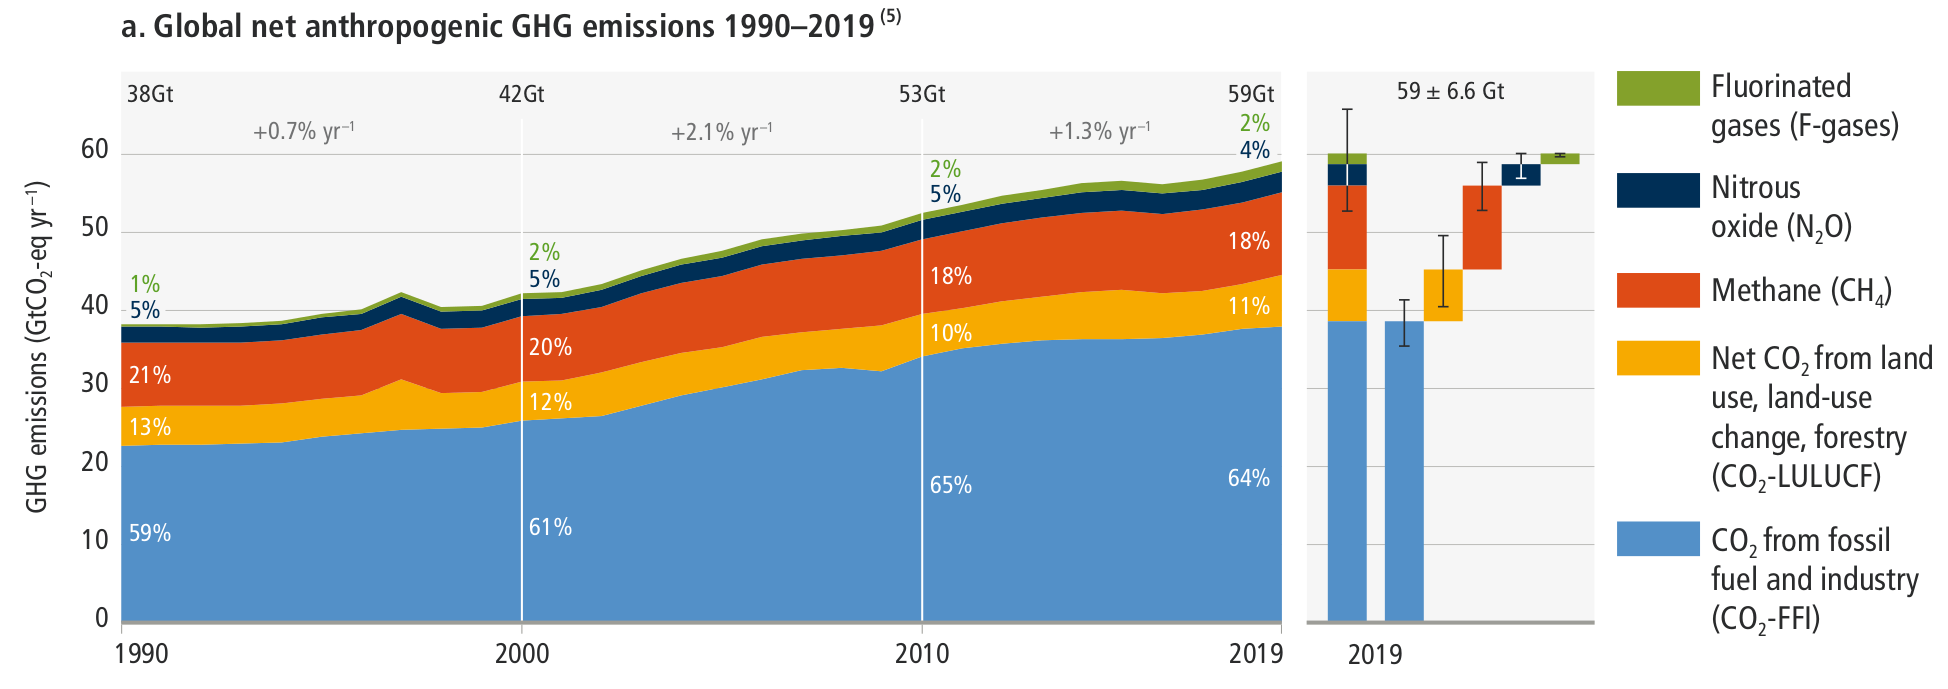
\includegraphics[width=1.0\textwidth]{plots/WG3_net_greenhouse_emissions.png}
      \end{center}   
    \end{columns}

  \end{scriptsize}
  \end{frame} 

  
%%%%%%%%%%%%%%%%%%%%%%%%%%%%%%%%%%%%%%%%%%%%%%%%%%%%%%%%%%%%%%%%%%%%%%%%%%%%%%%%%%
\begin{frame}
  \begin{scriptsize}

    \vspace{-0.1cm}
    \begin{columns}
      \column{0.52\textwidth}
      \begin{center}
          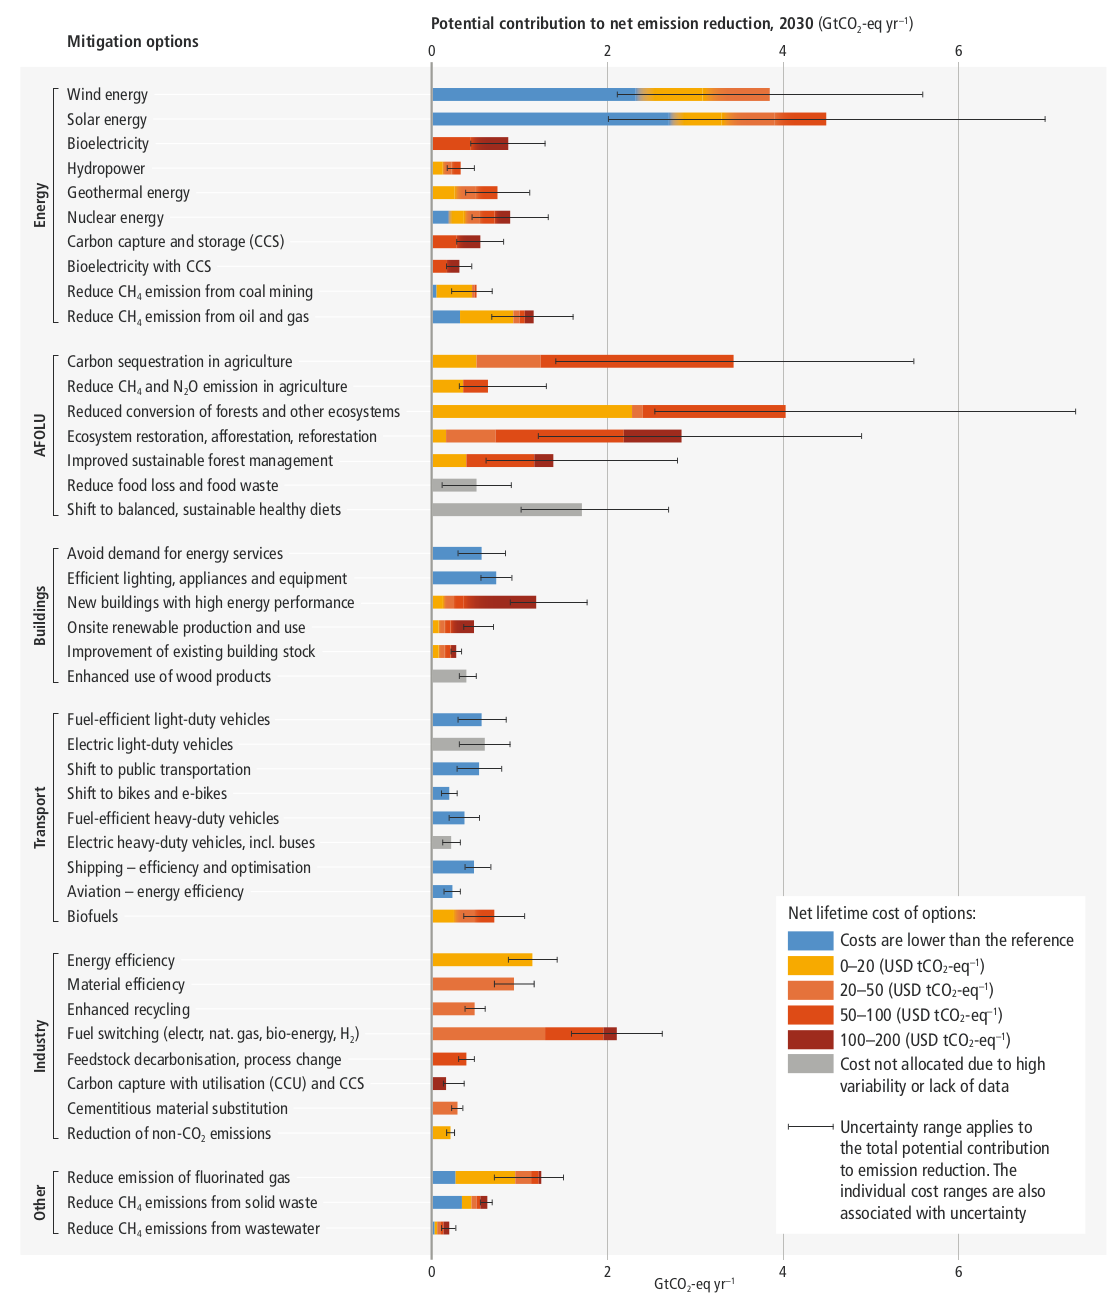
\includegraphics[width=1.0\textwidth]{plots/WG3_mitigation_options.png}
      \end{center}   

      \column{0.4\textwidth}
      \begin{itemize}\setlength\itemsep{1.9ex}        
        \item[o] \hhref{https://www.ipcc.ch/report/ar6/wg3/downloads/report/IPCC_AR6_WGIII_SPM.pdf}{IPCC  Mitigation of Climate Change}
      \end{itemize}
    \end{columns}

  \end{scriptsize}
  \end{frame} 

%%%%%%%%%%%%%%%%%%%%%%%%%%%%%%%%%%%%%%%%%%%%%%%%%%%%%%%%%%%%%%%%%%%%%%%%%%%%%%%%%%
\begin{frame}
  \begin{scriptsize}
              
  \vspace{-0.1cm}
  \begin{columns}
    \column{0.25\textwidth}
   Sources of CO$_2$ emissions in France:\\
   \vspace{0.1cm} 
   \hhref{https://rustem.web.cern.ch/climate/LeMondeClimateEmergencyFranceImpact.pdf}{Le Monde, May 30th, 2022}

    \column{0.55\textwidth}
    \begin{center}
        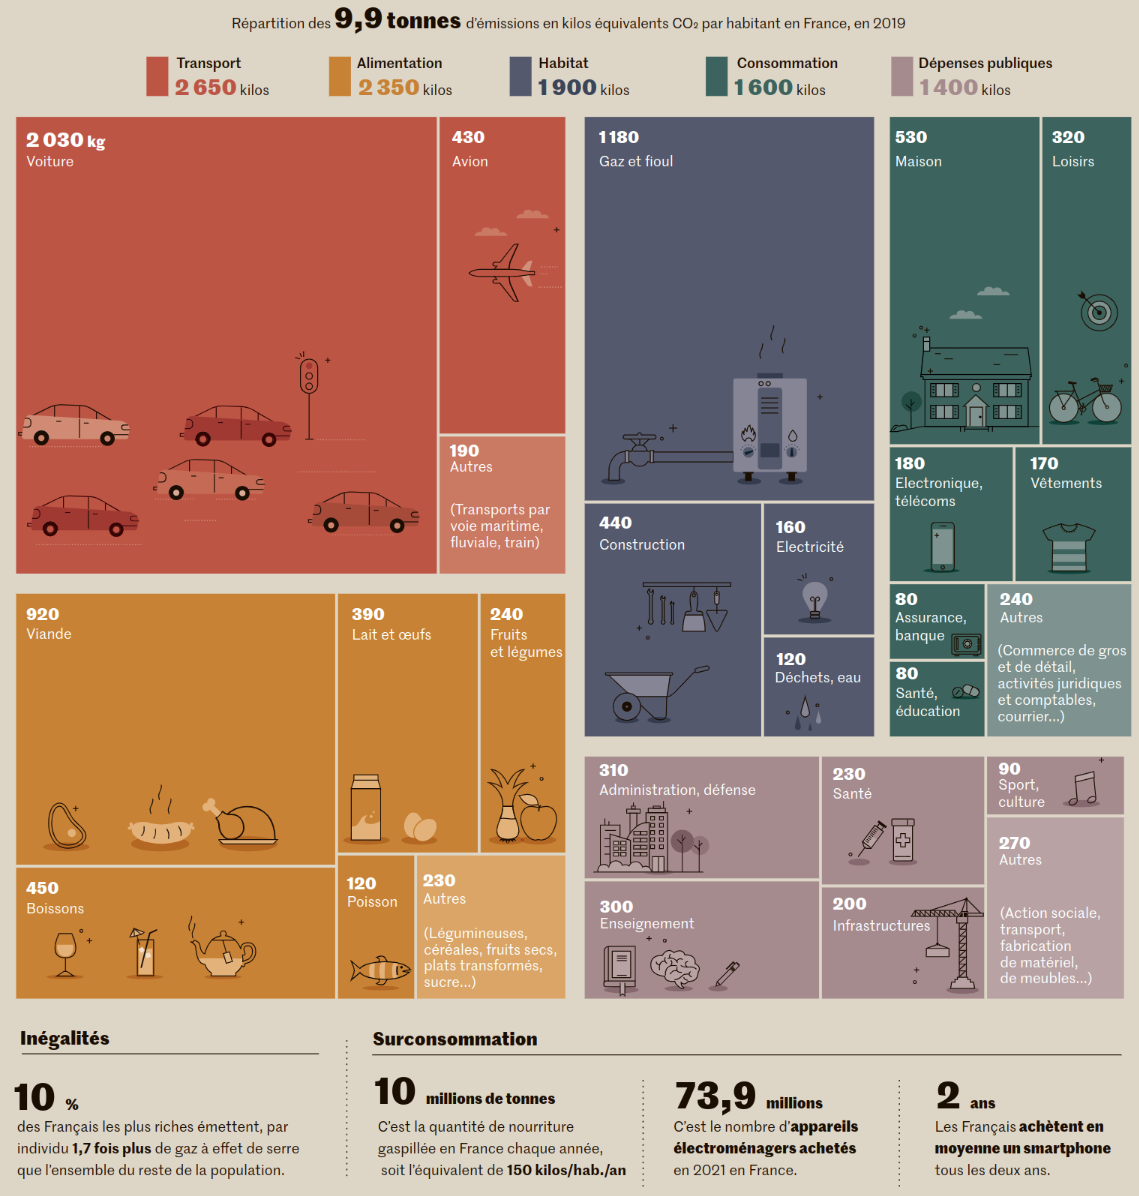
\includegraphics[width=1.0\textwidth]{plots/co2_breakdown.png}
    \end{center}
  \end{columns}

  \end{scriptsize}
  \end{frame}

  %%%%%%%%%%%%%%%%%%%%%%%%%%%%%%%%%%%%%%%%%%%%%%%%%%%%%%%%%%%%%%%%%%%%%%%%%%%%%%%%%%
  \begin{frame}
    \frametitle{\centerline{Summary}}
    \begin{footnotesize}
  
      \begin{columns}
        \column{1.0\textwidth}
        \begin{itemize}\setlength\itemsep{2.9ex}        
          \item[o] Global surface temperature will continue to increase until at least mid-century under all considered emissions scenarios.
  
          \item[o] Global warming of 1.5$^\circ$C and 2$^\circ$C will be exceeded during the 21st century, unless deep reductions in CO$_2$ and other greenhouse gas emissions occur in the coming decades.
  
          \item[o]  Extreme weather, rising seas and damaged ecosystems could threaten the safety and livelihoods of billions of people in the next decades. 

          \item[o] {\bf There could be 1.2 billion climate refugees by 2050} - \hhref{https://www.zurich.com/en/media/magazine/2022/there-could-be-1-2-billion-climate-refugees-by-2050-here-s-what-you-need-to-know}{Ecological Threat Register}
      \end{itemize}
      \end{columns}

  
    \end{footnotesize}
    \end{frame}  

%%%%%%%%%%%%%%%%%%%%%%%%%%%%%%%%%%%%%%%%%%%%%%%%%%%%%%%%%%%%%%%%%%%%%%%%%%%%%%%%%%
\end{document}

%%%%%%%%%%%%%%%%%%%%%%%%%%%%%%%%%%%%%%%%%%%%%%%%%%%%%%%%%%%%%%%%%%%%%%%%%%%%%%%%%%
%%%%%%%%%%%%%%%%%%%%%%%%%%%%%%%%%%%%%%%%%%%%%%%%%%%%%%%%%%%%%%%%%%%%%%%%%%%%%%%%%%


%%%%%%%%%%%%%%%%%%%%%%%%%%%%%%%%%%%%%%%%%%%%%%%%%%%%%%%%%%%%%%%%%%%%%%%%%%
%%%%%%%%%%%%%%%%%%%%%%%%%%%%%%%%%%%%%%%%%%%%%%%%%%%%%%%%%%%%%%%%%%%%%%%%%%
\begin{frame}
  \begin{small}
              
  \begin{columns}
  \column{0.9\textwidth}
  {\cb Intergovernmental Panel on Climate Change (IPCC) Assessment Report 6 (2021)}
    \begin{itemize}\setlength\itemsep{1.0ex}\footnotesize
      \item[1.]  \hhref{https://report.ipcc.ch/ar6wg2/pdf/IPCC_AR6_WGII_SummaryForPolicymakers.pdf}{Working Group II: Impacts, Adaptation and Vulnerability}
    \end{itemize}
  \end{columns}

  \end{small}
\end{frame}  

%%%%%%%%%%%%%%%%%%%%%%%%%%%%%%%%%%%%%%%%%%%%%%%%%%%%%%%%%%%%%%%%%%%%%%%%%%%%%%%%%%
\begin{frame}
  \frametitle{\centerline{\hhref{https://report.ipcc.ch/ar6wg2/pdf/IPCC_AR6_WGII_SummaryForPolicymakers.pdf}{IPCC Impacts, Adaptation and Vulnerability:} Climate change impact on natural ecosystems}}
  \begin{scriptsize}

    \begin{columns}
      \column{1.0\textwidth}
      \begin{itemize}\setlength\itemsep{1.9ex}        
        \item[o] A
      \end{itemize}

    \end{columns}

    \vspace{-0.1cm}
    \begin{columns}
      \column{0.9\textwidth}
      \begin{center}
          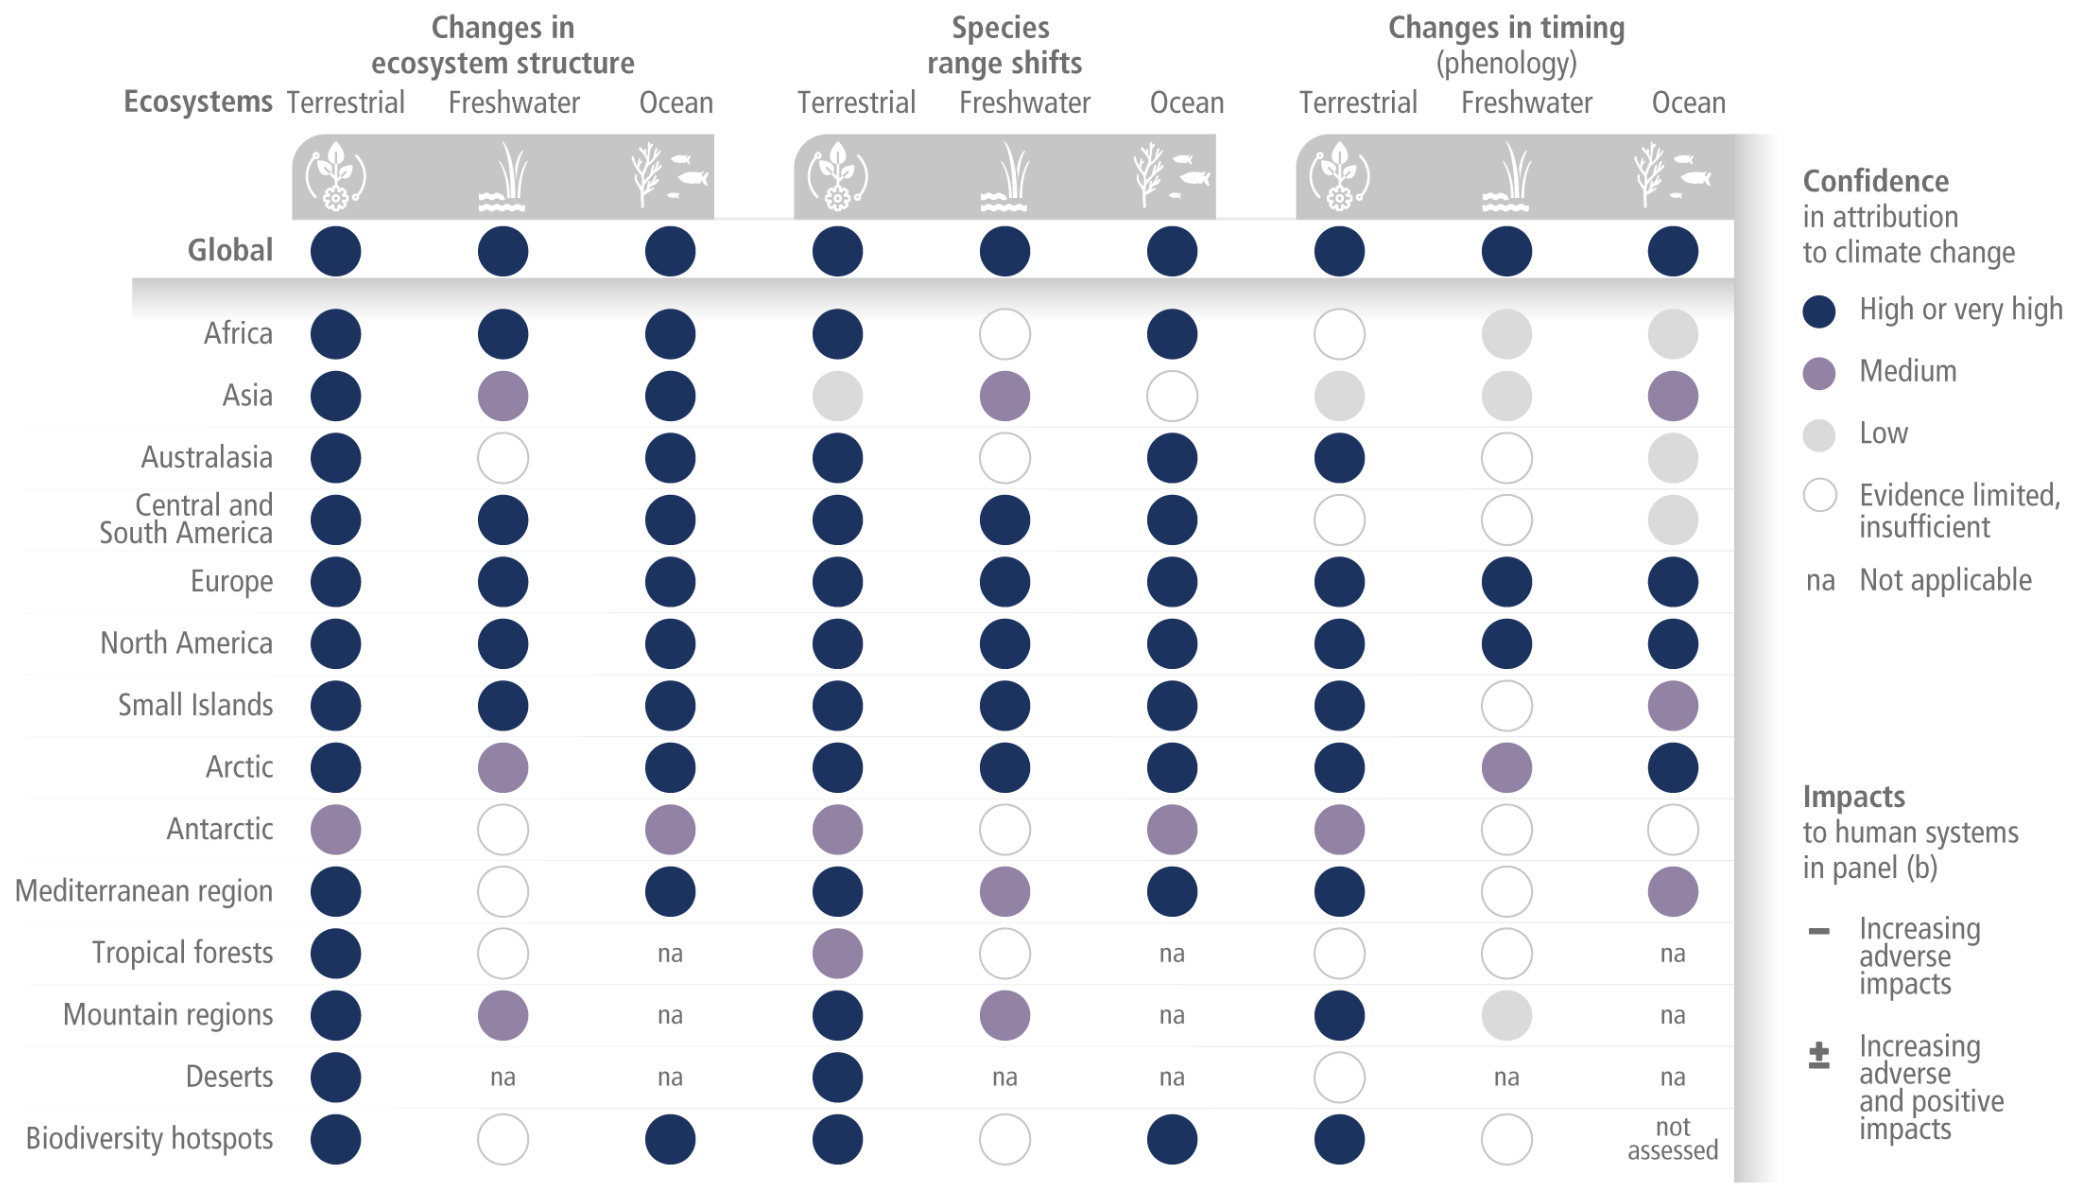
\includegraphics[width=1.0\textwidth]{plots/WG2_impact_on_ecosystems.png}
      \end{center}   
    \end{columns}

  \end{scriptsize}
  \end{frame}  

%%%%%%%%%%%%%%%%%%%%%%%%%%%%%%%%%%%%%%%%%%%%%%%%%%%%%%%%%%%%%%%%%%%%%%%%%%%%%%%%%%
\begin{frame}
  \frametitle{\centerline{\hhref{https://report.ipcc.ch/ar6wg2/pdf/IPCC_AR6_WGII_SummaryForPolicymakers.pdf}{IPCC Impacts, Adaptation and Vulnerability:} Climate change impact on human societies}}
  \begin{scriptsize}

    \begin{columns}
      \column{1.0\textwidth}
      \begin{itemize}\setlength\itemsep{1.9ex}        
        \item[o] B
      \end{itemize}

    \end{columns}

    \vspace{-0.1cm}
    \begin{columns}
      \column{0.9\textwidth}
      \begin{center}
          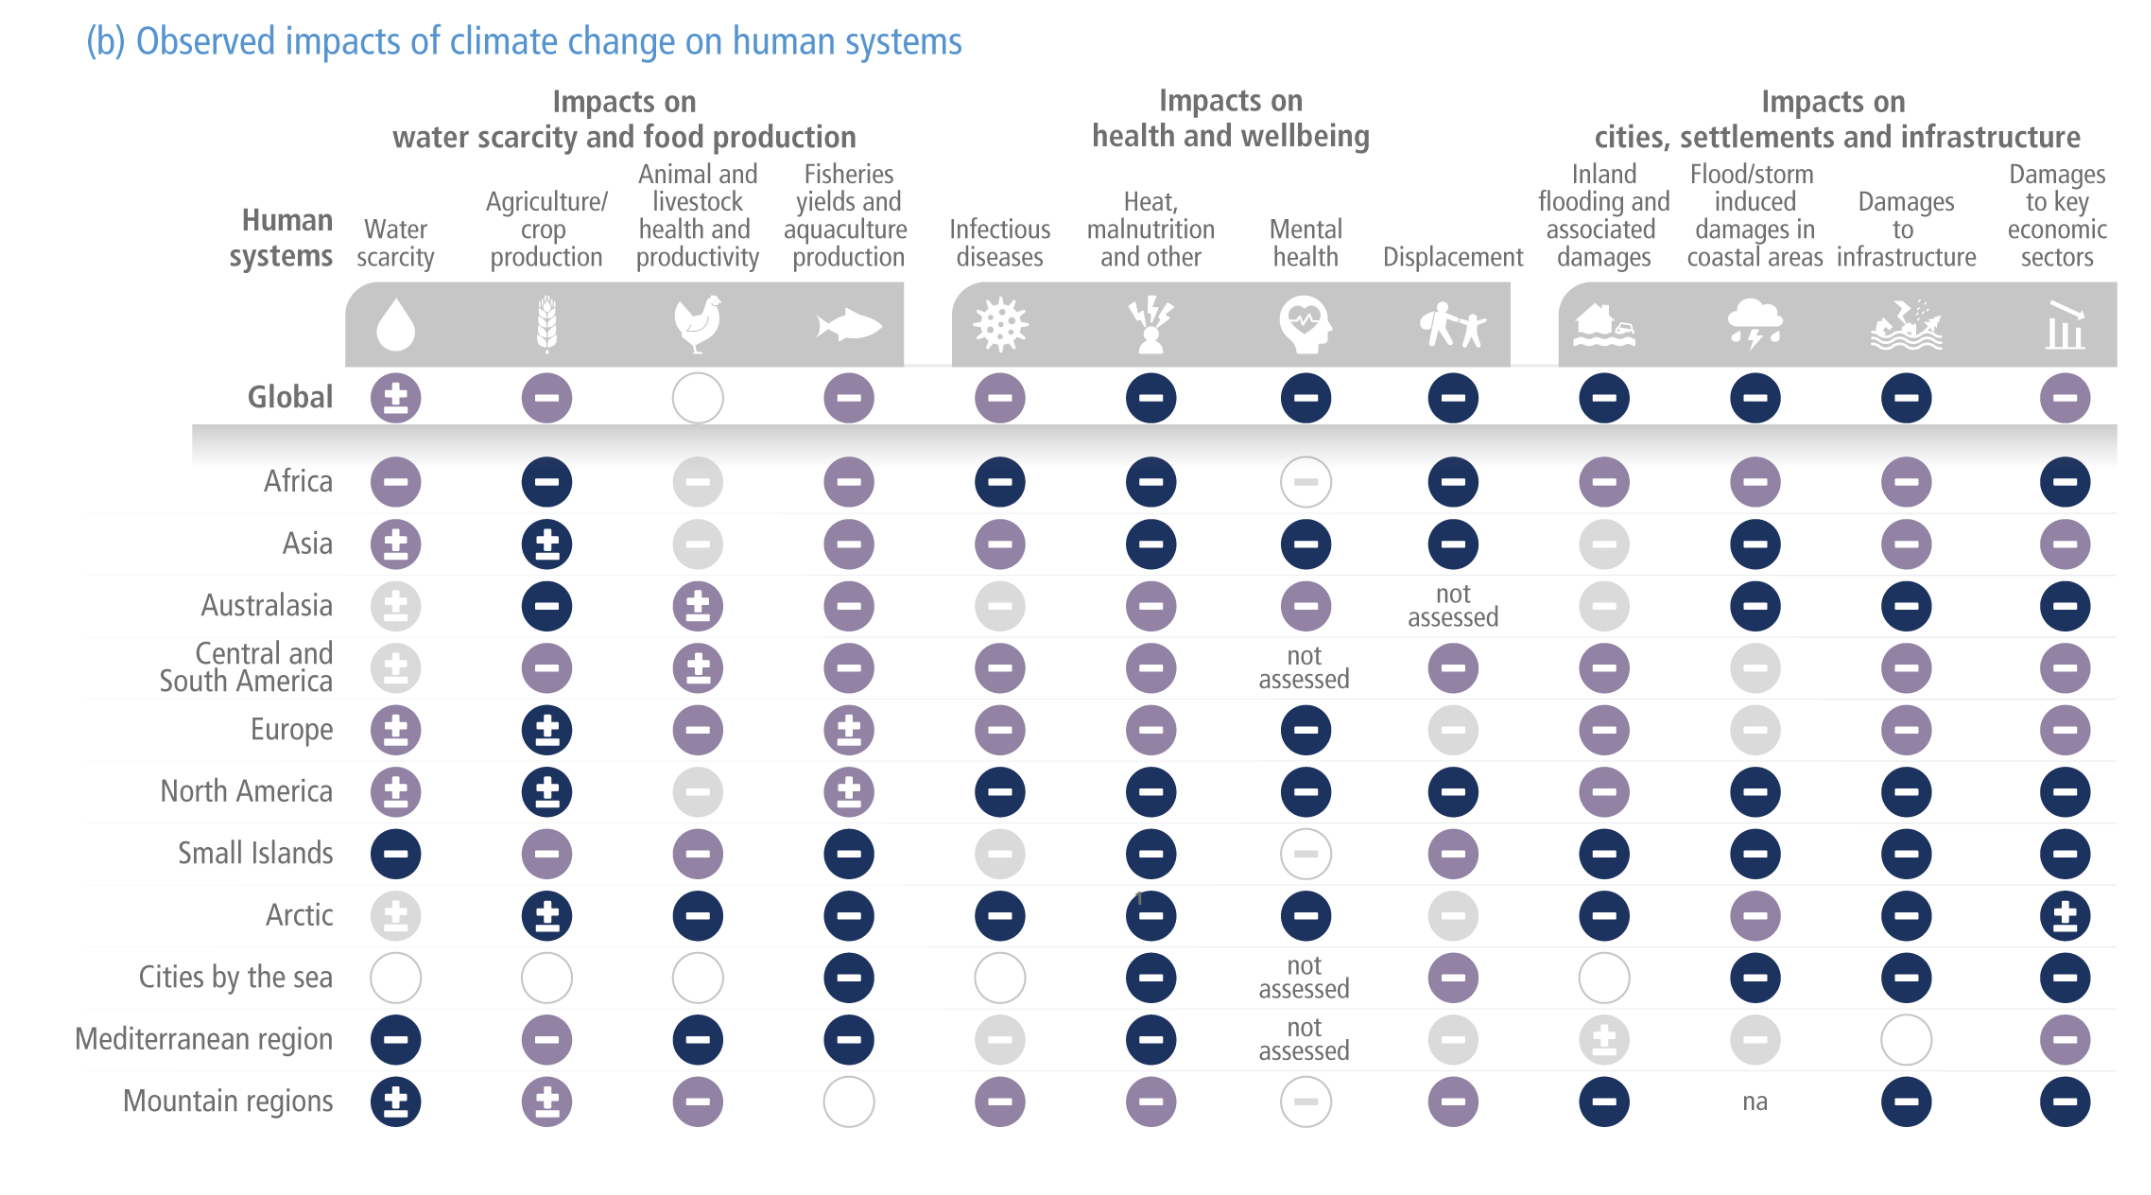
\includegraphics[width=1.0\textwidth]{plots/WG2_impact_on_society.png}
      \end{center}   
    \end{columns}

  \end{scriptsize}
  \end{frame}  

%%%%%%%%%%%%%%%%%%%%%%%%%%%%%%%%%%%%%%%%%%%%%%%%%%%%%%%%%%%%%%%%%%%%%%%%%%%%%%%%%%
%%%%%%%%%%%%%%%%%%%%%%%%%%%%%%%%%%%%%%%%%%%%%%%%%%%%%%%%%%%%%%%%%%%%%%%%%%%%%%%%%%


%%%%%%%%%%%%%%%%%%%%%%%%%%%%%%%%%%%%%%%%%%%%%%%%%%%%%%%%%%%%%%%%%%%%%%%%%%
%%%%%%%%%%%%%%%%%%%%%%%%%%%%%%%%%%%%%%%%%%%%%%%%%%%%%%%%%%%%%%%%%%%%%%%%%%
\begin{frame}
  \begin{small}
              
  \begin{columns}
  \column{0.9\textwidth}
  {\cb Intergovernmental Panel on Climate Change (IPCC) Assessment Report 6 (2021)}
    \begin{itemize}\setlength\itemsep{1.0ex}\footnotesize
      \item[1.]  \hhref{https://www.ipcc.ch/report/ar6/wg3/downloads/report/IPCC_AR6_WGIII_SPM.pdf}{Working Group III:  Mitigation of Climate Change}
    \end{itemize}
  \end{columns}

  \end{small}
\end{frame}  

%%%%%%%%%%%%%%%%%%%%%%%%%%%%%%%%%%%%%%%%%%%%%%%%%%%%%%%%%%%%%%%%%%%%%%%%%%%%%%%%%%
\begin{frame}
  \begin{scriptsize}

    \vspace{-0.1cm}
    \begin{columns}
      \column{0.43\textwidth}
      \begin{center}
          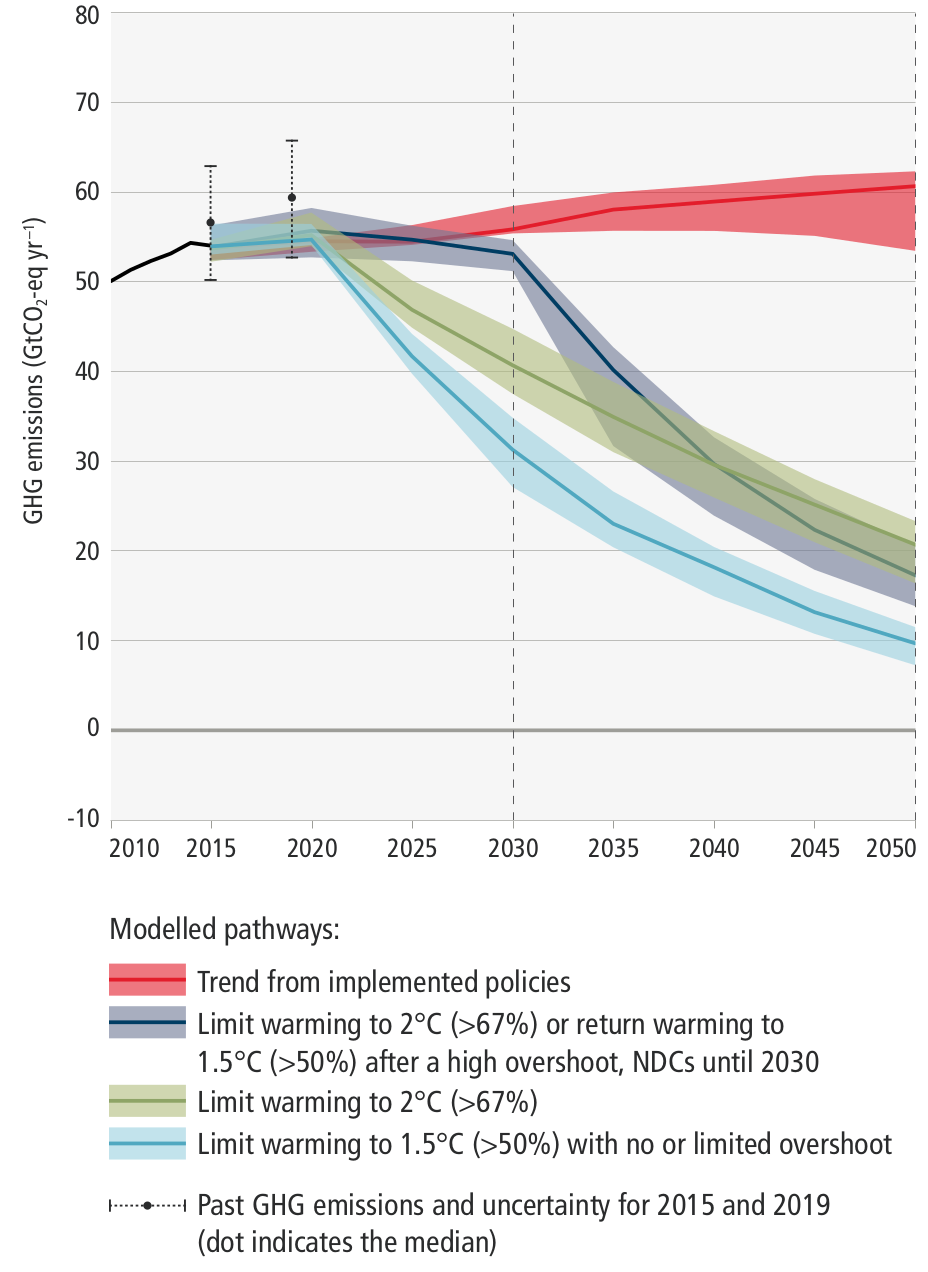
\includegraphics[width=1.0\textwidth]{plots/WG3_global_GHG_emissions.png}
      \end{center}  
      
      \column{0.5\textwidth}
      \begin{itemize}\setlength\itemsep{1.9ex}        
        \item[o] \hhref{https://www.ipcc.ch/report/ar6/wg3/downloads/report/IPCC_AR6_WGIII_SPM.pdf}{IPCC  Mitigation of Climate Change:}
      \end{itemize}

    \end{columns}

  \end{scriptsize}
  \end{frame}  

%%%%%%%%%%%%%%%%%%%%%%%%%%%%%%%%%%%%%%%%%%%%%%%%%%%%%%%%%%%%%%%%%%%%%%%%%%%%%%%%%%
\begin{frame}
  \frametitle{\centerline{\hhref{https://www.ipcc.ch/report/ar6/wg3/downloads/report/IPCC_AR6_WGIII_SPM.pdf}{IPCC  Mitigation of Climate Change:} Climate change impact on natural ecosystems}}
  \begin{scriptsize}

    \begin{columns}
      \column{1.0\textwidth}
      \begin{itemize}\setlength\itemsep{1.9ex}        
        \item[o] A
      \end{itemize}

    \end{columns}

    \vspace{-0.1cm}
    \begin{columns}
      \column{0.99\textwidth}
      \begin{center}
          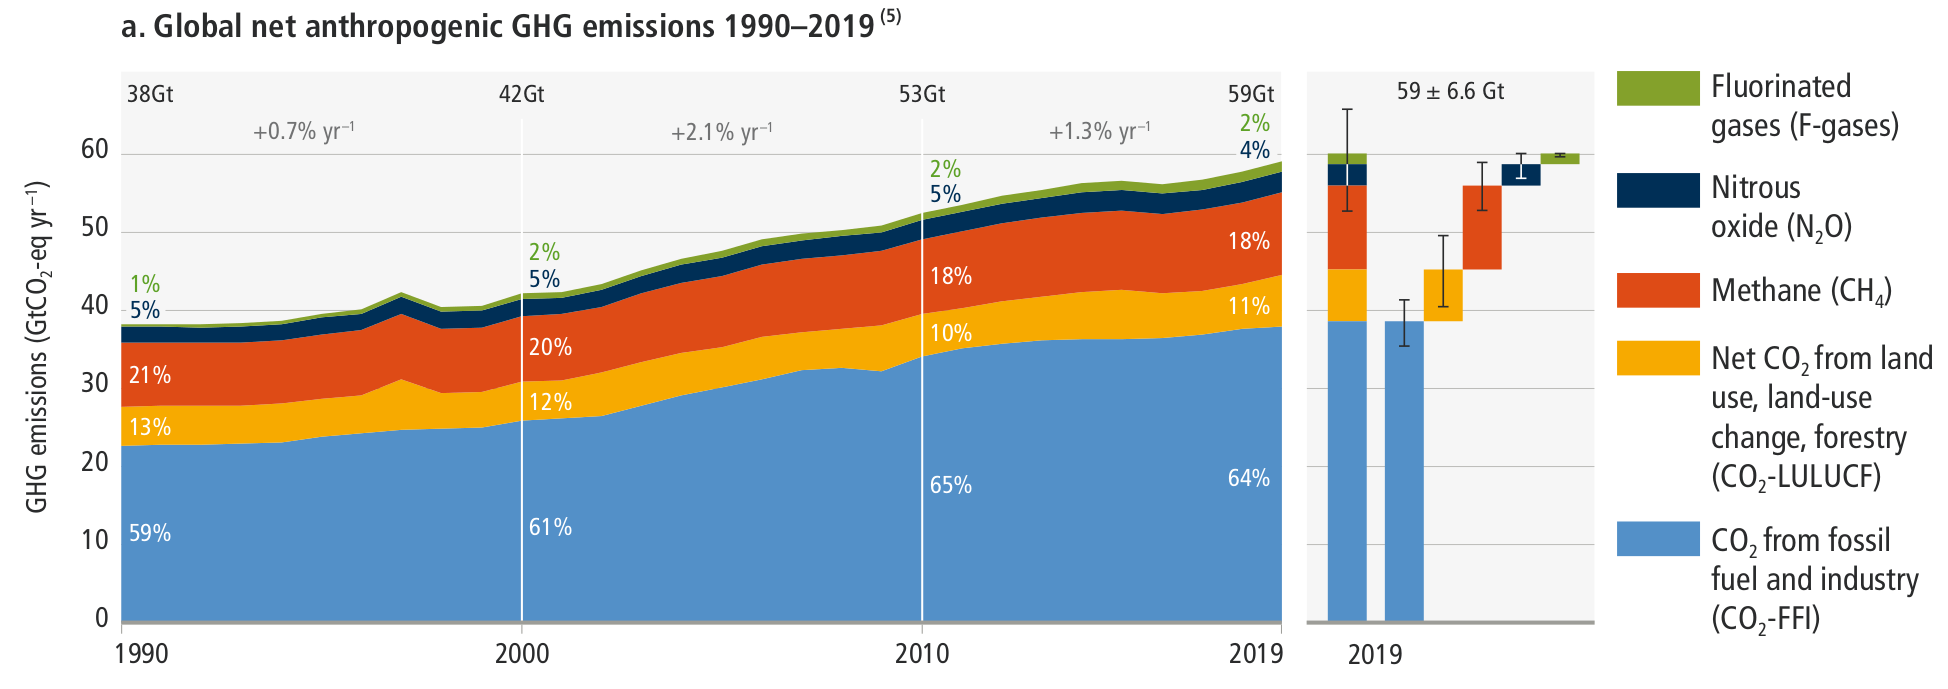
\includegraphics[width=1.0\textwidth]{plots/WG3_net_greenhouse_emissions.png}
      \end{center}   
    \end{columns}

  \end{scriptsize}
  \end{frame} 

  
%%%%%%%%%%%%%%%%%%%%%%%%%%%%%%%%%%%%%%%%%%%%%%%%%%%%%%%%%%%%%%%%%%%%%%%%%%%%%%%%%%
\begin{frame}
  \begin{scriptsize}

    \vspace{-0.1cm}
    \begin{columns}
      \column{0.52\textwidth}
      \begin{center}
          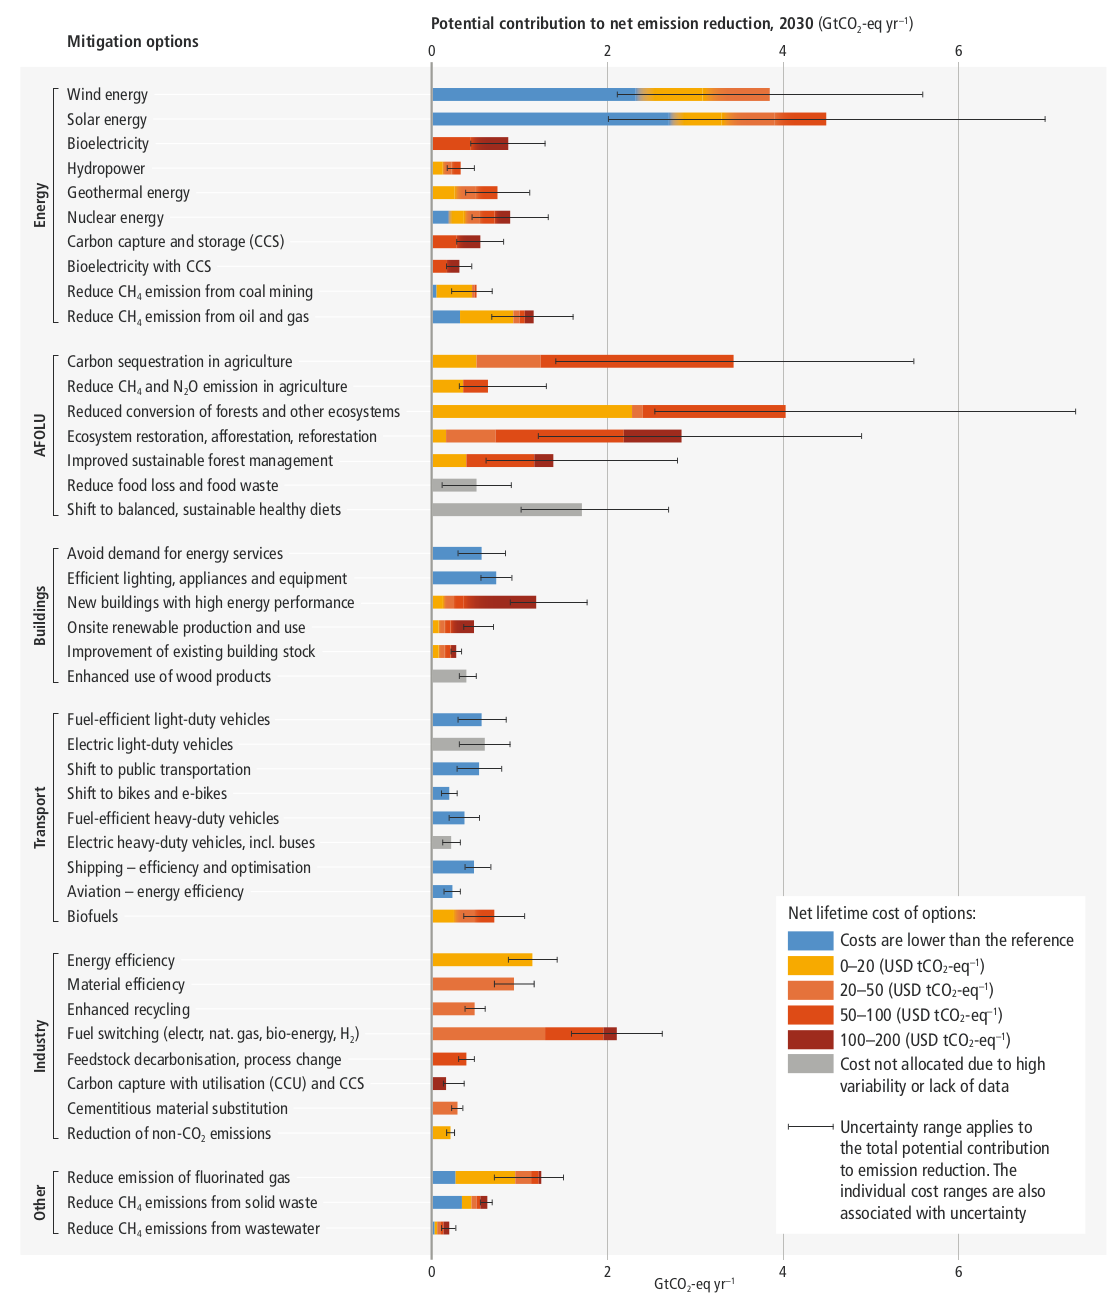
\includegraphics[width=1.0\textwidth]{plots/WG3_mitigation_options.png}
      \end{center}   

      \column{0.4\textwidth}
      \begin{itemize}\setlength\itemsep{1.9ex}        
        \item[o] \hhref{https://www.ipcc.ch/report/ar6/wg3/downloads/report/IPCC_AR6_WGIII_SPM.pdf}{IPCC  Mitigation of Climate Change}
      \end{itemize}
    \end{columns}

  \end{scriptsize}
  \end{frame} 

%%%%%%%%%%%%%%%%%%%%%%%%%%%%%%%%%%%%%%%%%%%%%%%%%%%%%%%%%%%%%%%%%%%%%%%%%%%%%%%%%%
\begin{frame}
  \begin{scriptsize}
              
  \vspace{-0.1cm}
  \begin{columns}
    \column{0.25\textwidth}
   Sources of CO$_2$ emissions in France:\\
   \vspace{0.1cm} 
   \hhref{https://rustem.web.cern.ch/climate/LeMondeClimateEmergencyFranceImpact.pdf}{Le Monde, May 30th, 2022}

    \column{0.55\textwidth}
    \begin{center}
        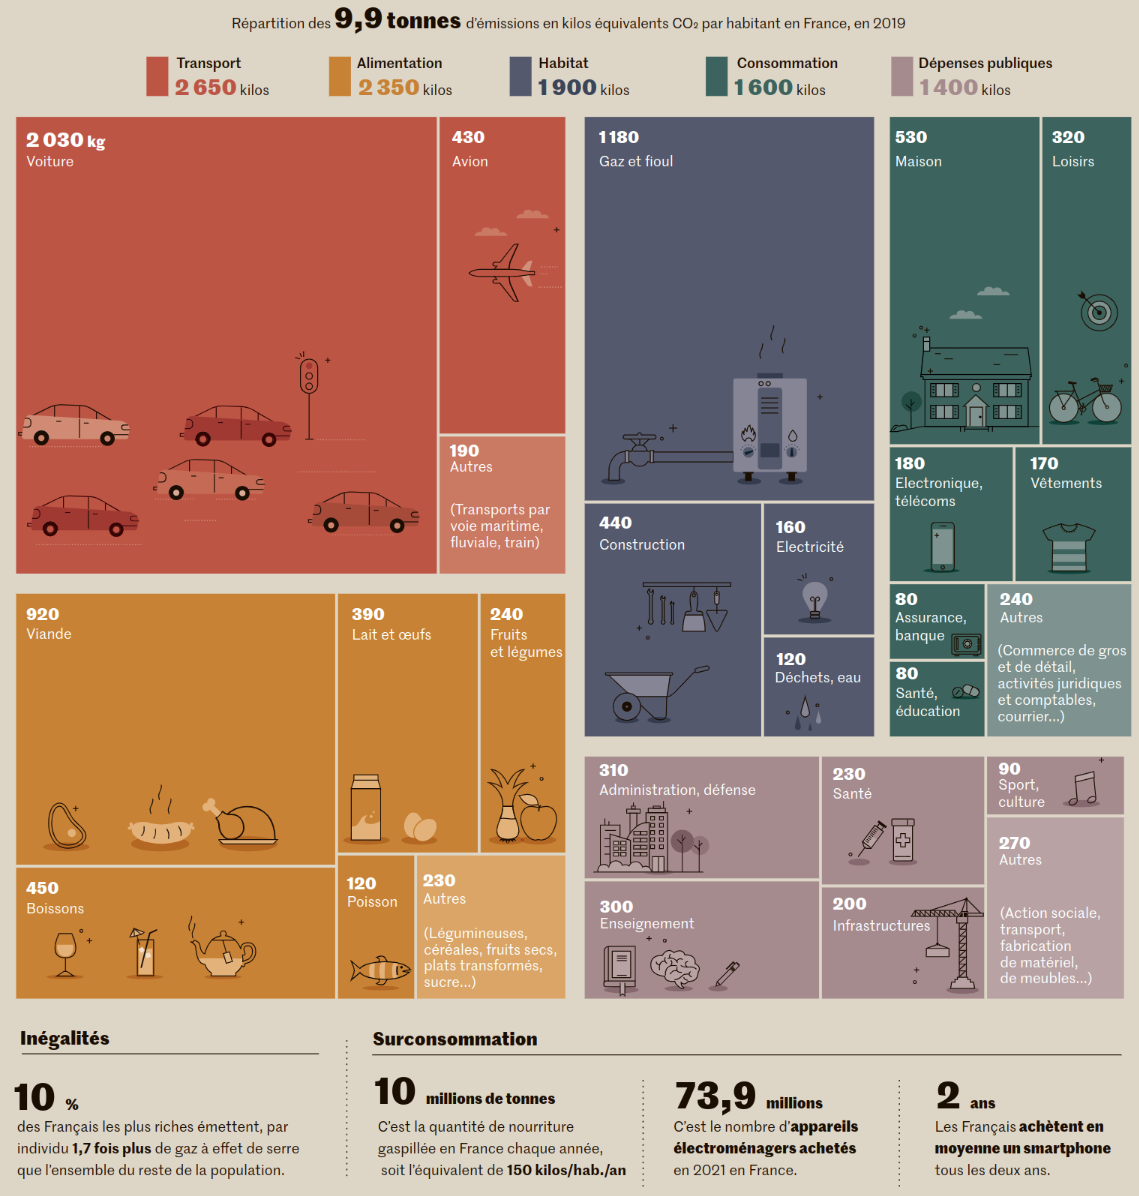
\includegraphics[width=1.0\textwidth]{plots/co2_breakdown.png}
    \end{center}
  \end{columns}

  \end{scriptsize}
  \end{frame}

%%%%%%%%%%%%%%%%%%%%%%%%%%%%%%%%%%%%%%%%%%%%%%%%%%%%%%%%%%%%%%%%%%%%%%%%%%%%%%%%%%
\begin{frame}
  \frametitle{\centerline{Summary}}
  \begin{footnotesize}

    \begin{columns}
      \column{1.0\textwidth}
      \begin{itemize}\setlength\itemsep{2.9ex}        
        \item[o] Global surface temperature will continue to increase until at least mid-century under all considered emissions scenarios.

        \item[o] Global warming of 1.5$^\circ$C and 2$^\circ$C will be exceeded during the 21st century, unless deep reductions in CO$_2$ and other greenhouse gas emissions occur in the coming decades.

        \item[o] Ensuing extreme weather, rising seas and damaged ecosystems could threaten the safety and livelihoods of billions. 

        \item[o] \hhref{https://www.zurich.com/en/media/magazine/2022/there-could-be-1-2-billion-climate-refugees-by-2050-here-s-what-you-need-to-know}{There could be 1.2 billion climate refugees by 2050.}

        \item[o] Please help to improve these slides: \hhref{https://github.com/rustemos/ClimateSummary2022}{https://github.com/rustemos/ClimateSummary2022}
    \end{itemize}
    \end{columns}


  \end{footnotesize}
\end{frame}  

%%%%%%%%%%%%%%%%%%%%%%%%%%%%%%%%%%%%%%%%%%%%%%%%%%%%%%%%%%%%%%%%%%%%%%%%%%%%%%%%%%
\end{document}